% Options for packages loaded elsewhere
\PassOptionsToPackage{unicode}{hyperref}
\PassOptionsToPackage{hyphens}{url}
\documentclass[
  english,
]{article}
\usepackage{xcolor}
\usepackage{amsmath,amssymb}
\setcounter{secnumdepth}{-\maxdimen} % remove section numbering
\usepackage{iftex}
\ifPDFTeX
  \usepackage[T1]{fontenc}
  \usepackage[utf8]{inputenc}
  \usepackage{textcomp} % provide euro and other symbols
\else % if luatex or xetex
  \usepackage{unicode-math} % this also loads fontspec
  \defaultfontfeatures{Scale=MatchLowercase}
  \defaultfontfeatures[\rmfamily]{Ligatures=TeX,Scale=1}
\fi
\usepackage{lmodern}
\ifPDFTeX\else
  % xetex/luatex font selection
\fi
% Use upquote if available, for straight quotes in verbatim environments
\IfFileExists{upquote.sty}{\usepackage{upquote}}{}
\IfFileExists{microtype.sty}{% use microtype if available
  \usepackage[]{microtype}
  \UseMicrotypeSet[protrusion]{basicmath} % disable protrusion for tt fonts
}{}
\makeatletter
\@ifundefined{KOMAClassName}{% if non-KOMA class
  \IfFileExists{parskip.sty}{%
    \usepackage{parskip}
  }{% else
    \setlength{\parindent}{0pt}
    \setlength{\parskip}{6pt plus 2pt minus 1pt}}
}{% if KOMA class
  \KOMAoptions{parskip=half}}
\makeatother
\usepackage{color}
\usepackage{fancyvrb}
\newcommand{\VerbBar}{|}
\newcommand{\VERB}{\Verb[commandchars=\\\{\}]}
\DefineVerbatimEnvironment{Highlighting}{Verbatim}{commandchars=\\\{\}}
% Add ',fontsize=\small' for more characters per line
\newenvironment{Shaded}{}{}
\newcommand{\AlertTok}[1]{\textcolor[rgb]{1.00,0.00,0.00}{\textbf{#1}}}
\newcommand{\AnnotationTok}[1]{\textcolor[rgb]{0.38,0.63,0.69}{\textbf{\textit{#1}}}}
\newcommand{\AttributeTok}[1]{\textcolor[rgb]{0.49,0.56,0.16}{#1}}
\newcommand{\BaseNTok}[1]{\textcolor[rgb]{0.25,0.63,0.44}{#1}}
\newcommand{\BuiltInTok}[1]{\textcolor[rgb]{0.00,0.50,0.00}{#1}}
\newcommand{\CharTok}[1]{\textcolor[rgb]{0.25,0.44,0.63}{#1}}
\newcommand{\CommentTok}[1]{\textcolor[rgb]{0.38,0.63,0.69}{\textit{#1}}}
\newcommand{\CommentVarTok}[1]{\textcolor[rgb]{0.38,0.63,0.69}{\textbf{\textit{#1}}}}
\newcommand{\ConstantTok}[1]{\textcolor[rgb]{0.53,0.00,0.00}{#1}}
\newcommand{\ControlFlowTok}[1]{\textcolor[rgb]{0.00,0.44,0.13}{\textbf{#1}}}
\newcommand{\DataTypeTok}[1]{\textcolor[rgb]{0.56,0.13,0.00}{#1}}
\newcommand{\DecValTok}[1]{\textcolor[rgb]{0.25,0.63,0.44}{#1}}
\newcommand{\DocumentationTok}[1]{\textcolor[rgb]{0.73,0.13,0.13}{\textit{#1}}}
\newcommand{\ErrorTok}[1]{\textcolor[rgb]{1.00,0.00,0.00}{\textbf{#1}}}
\newcommand{\ExtensionTok}[1]{#1}
\newcommand{\FloatTok}[1]{\textcolor[rgb]{0.25,0.63,0.44}{#1}}
\newcommand{\FunctionTok}[1]{\textcolor[rgb]{0.02,0.16,0.49}{#1}}
\newcommand{\ImportTok}[1]{\textcolor[rgb]{0.00,0.50,0.00}{\textbf{#1}}}
\newcommand{\InformationTok}[1]{\textcolor[rgb]{0.38,0.63,0.69}{\textbf{\textit{#1}}}}
\newcommand{\KeywordTok}[1]{\textcolor[rgb]{0.00,0.44,0.13}{\textbf{#1}}}
\newcommand{\NormalTok}[1]{#1}
\newcommand{\OperatorTok}[1]{\textcolor[rgb]{0.40,0.40,0.40}{#1}}
\newcommand{\OtherTok}[1]{\textcolor[rgb]{0.00,0.44,0.13}{#1}}
\newcommand{\PreprocessorTok}[1]{\textcolor[rgb]{0.74,0.48,0.00}{#1}}
\newcommand{\RegionMarkerTok}[1]{#1}
\newcommand{\SpecialCharTok}[1]{\textcolor[rgb]{0.25,0.44,0.63}{#1}}
\newcommand{\SpecialStringTok}[1]{\textcolor[rgb]{0.73,0.40,0.53}{#1}}
\newcommand{\StringTok}[1]{\textcolor[rgb]{0.25,0.44,0.63}{#1}}
\newcommand{\VariableTok}[1]{\textcolor[rgb]{0.10,0.09,0.49}{#1}}
\newcommand{\VerbatimStringTok}[1]{\textcolor[rgb]{0.25,0.44,0.63}{#1}}
\newcommand{\WarningTok}[1]{\textcolor[rgb]{0.38,0.63,0.69}{\textbf{\textit{#1}}}}
\usepackage{longtable,booktabs,array}
\newcounter{none} % for unnumbered tables
\usepackage{calc} % for calculating minipage widths
% Correct order of tables after \paragraph or \subparagraph
\usepackage{etoolbox}
\makeatletter
\patchcmd\longtable{\par}{\if@noskipsec\mbox{}\fi\par}{}{}
\makeatother
% Allow footnotes in longtable head/foot
\IfFileExists{footnotehyper.sty}{\usepackage{footnotehyper}}{\usepackage{footnote}}
\makesavenoteenv{longtable}
\usepackage{graphicx}
\makeatletter
\newsavebox\pandoc@box
\newcommand*\pandocbounded[1]{% scales image to fit in text height/width
  \sbox\pandoc@box{#1}%
  \Gscale@div\@tempa{\textheight}{\dimexpr\ht\pandoc@box+\dp\pandoc@box\relax}%
  \Gscale@div\@tempb{\linewidth}{\wd\pandoc@box}%
  \ifdim\@tempb\p@<\@tempa\p@\let\@tempa\@tempb\fi% select the smaller of both
  \ifdim\@tempa\p@<\p@\scalebox{\@tempa}{\usebox\pandoc@box}%
  \else\usebox{\pandoc@box}%
  \fi%
}
% Set default figure placement to htbp
\def\fps@figure{htbp}
\makeatother
\ifLuaTeX
\usepackage[bidi=basic,shorthands=off]{babel}
\else
\usepackage[bidi=default,shorthands=off]{babel}
\fi
\ifLuaTeX
  \usepackage{selnolig} % disable illegal ligatures
\fi
\setlength{\emergencystretch}{3em} % prevent overfull lines
\providecommand{\tightlist}{%
  \setlength{\itemsep}{0pt}\setlength{\parskip}{0pt}}
\usepackage{bookmark}
\IfFileExists{xurl.sty}{\usepackage{xurl}}{} % add URL line breaks if available
\urlstyle{same}
\hypersetup{
  pdftitle={Tree of Thoughts Meets Hugging Face Agents},
  pdflang={en},
  hidelinks,
  pdfcreator={LaTeX via pandoc}}

\title{Tree of Thoughts Meets Hugging Face Agents}
\author{}
\date{}

\begin{document}
\maketitle

\section{Tree of Thoughts Meets Hugging Face
Agents}\label{tree-of-thoughts-meets-hugging-face-agents}

A Survey of Tree of Thoughts and Hugging Face Agent Frameworks

\textbf{Authors:} Michael Leydon\textsuperscript{1}

\begin{enumerate}
\tightlist
\item
  \textbf{1} Independent Researcher, United States
\end{enumerate}

\textbf{Author links (Michael Leydon):}
\href{https://www.linkedin.com/in/michael-leydon/}{linkedin.com/in/michael-leydon};
\href{https://www.quiznat.com/}{quiznat.com}

\textbf{Version:} v1.1 -- Final pre-submission clean (19 February 2026)

\textbf{Submission date:} TBD

\textbf{arXiv categories:} cs.AI (primary); cs.CL (cross-list), cs.LG
(optional cross-list)

Abstract

Large Language Models (LLMs) have demonstrated remarkable capabilities
across diverse tasks, yet their reasoning remains fundamentally
linear---generating thoughts token-by-token without the ability to
explore alternatives, backtrack from errors, or evaluate multiple
solution paths. This limitation constrains their effectiveness on
complex multi-step problems requiring deliberation and planning.
Concurrently, the emergence of AI agent frameworks has enabled LLMs to
interact with external tools and execute actions autonomously, but these
systems often struggle with strategic reasoning and error recovery {[}1,
3, 4, 6, 8, 9{]}.

This paper presents a systematic synthesis of two developments in
artificial intelligence: Tree of Thoughts (ToT) reasoning and the
Hugging Face agent ecosystem. We examine how structured search over
reasoning paths can be integrated with accessible agent frameworks to
create more robust autonomous systems. Through technical analysis,
implementation patterns, and benchmark context from prior literature, we
describe where systematic exploration can improve complex reasoning
while also introducing cost and latency trade-offs {[}1, 2, 10, 11, 12,
26{]}.

Our contributions include: (1) a thorough theoretical and practical
examination of Tree of Thoughts as both a reasoning paradigm and
implementation strategy; (2) detailed documentation of Hugging
Face\textquotesingle s agent frameworks, including the Agent Course
educational pathway and the smolagents library; (3) architectural
patterns for integrating ToT reasoning with CodeAgent and MultiStepAgent
implementations; (4) case-study walkthroughs across financial analysis,
creative content generation, and software engineering; and (5) practical
implementation strategies, optimization techniques, and deployment
patterns.

This work summarizes published research and implementation patterns so
researchers and practitioners can evaluate structured-reasoning agent
designs with clear evidence boundaries.

\subsection{Note on Authorship}\label{note-on-authorship}

Michael Leydon is the sole listed author of this manuscript and accepts
full responsibility for final editorial review, factual accuracy, and
submission accountability.

This manuscript workflow included autonomous system assistance in early
drafting and human-led revision, verification, and final approval.
Non-human systems are treated as contributors to process, while
scholarly accountability for claims and submission remains with the
listed human author.

\textbf{Keywords:} Tree of Thoughts, LLM reasoning, AI agents, Hugging
Face agents, smolagents, tool-augmented reasoning, survey methodology

\textbf{Scope and evidence note.} This document is a technical overview
and synthesis. It combines literature findings with implementation
guidance. Reported benchmark gains (for example, ToT results on Game of
24) are attributed to cited prior work unless explicitly marked as
original measurements.

\begin{center}\rule{0.5\linewidth}{0.5pt}\end{center}

\subsection{0. Scope and Claim
Boundaries}\label{scope-and-claim-boundaries}

\begin{itemize}
\tightlist
\item
  This paper is primarily a survey-style synthesis rather than a
  standalone benchmark paper.
\item
  Code snippets are mixed: some are runnable examples, while others are
  architectural sketches.
\item
  Pseudo-code and illustrative snippets are labeled explicitly in
  relevant sections.
\item
  Non-empirical examples are included only as synthetic walkthroughs and
  are labeled accordingly.
\end{itemize}

\subsubsection{0.1 Survey Research
Questions}\label{survey-research-questions}

This survey is organized around the following research questions (RQs):

\begin{itemize}
\tightlist
\item
  \textbf{RQ1:} What technical mechanisms define Tree-of-Thought-style
  reasoning for LLM systems (generation, evaluation, search, and
  stopping)?
\item
  \textbf{RQ2:} What empirical evidence exists for ToT-family methods
  across benchmark categories relevant to agentic reasoning?
\item
  \textbf{RQ3:} How do Hugging Face agent frameworks expose integration
  points for structured reasoning strategies?
\item
  \textbf{RQ4:} What are the main methodological gaps that must be
  closed for reproducible ToT-agent claims?
\end{itemize}

\subsubsection{0.2 Survey Methodology and
Protocol}\label{survey-methodology-and-protocol}

We follow a transparent evidence-synthesis workflow adapted from
PRISMA-style reporting {[}27{]} and software-engineering evidence
synthesis guidance {[}28, 29, 30{]}. Because this is a computer-science
technical survey rather than a medical meta-analysis, we apply the
reporting principles (search transparency, screening traceability, and
extraction reproducibility) without imposing clinical effect-size
assumptions.

\textbf{Protocol scope (this version):} This manuscript freezes a
core-corpus selection run (Run ID: TOT-HF-SURVEY-2026-02-19) anchored by
the records listed in Section 8. Fixed selection counts and exclusion
reasons are reported in Appendix D, and the corresponding extraction
schema is reported in Appendix E.

Because this survey targets a narrow synthesis question (ToT-style
reasoning integrated with Hugging Face agent frameworks), the frozen run
begins from an explicitly pre-curated candidate set before full-text
screening. Query families, screening decisions, and extraction fields
are documented in Appendix D and Appendix E so this scope choice is
transparent and auditable.

\paragraph{0.2.1 Sources and Search
Strategy}\label{sources-and-search-strategy}

Primary sources for the final frozen search protocol are: arXiv, ACL
Anthology (where applicable), major ML conference proceedings
(NeurIPS/ICLR/ICML), ACM Digital Library, IEEE Xplore, and official
framework documentation for implementation-level claims {[}10, 11,
13{]}.

\textbf{Core query families (representative):}

\begin{itemize}
\tightlist
\item
  \texttt{("tree\ of\ thoughts"\ OR\ "tree-of-thought"\ OR\ "thought\ search")\ AND\ ("large\ language\ model"\ OR\ LLM)}
\item
  \texttt{("llm\ agent"\ OR\ "tool\ use"\ OR\ "tool-augmented")\ AND\ (reasoning\ OR\ planning\ OR\ search)}
\item
  \texttt{("smolagents"\ OR\ "hugging\ face\ agents"\ OR\ "CodeAgent"\ OR\ "MultiStepAgent")\ AND\ (planning\ OR\ reasoning)}
\end{itemize}

\paragraph{0.2.2 Inclusion and Exclusion
Criteria}\label{inclusion-and-exclusion-criteria}

\textbf{Inclusion:} peer-reviewed papers or clearly attributable
technical reports with reproducible method descriptions; benchmark
definitions sufficiently detailed to interpret results; and
framework/documentation sources required for implementation claims
{[}27, 28, 29, 30{]}.

\textbf{Exclusion:} marketing/blog-only claims without method
transparency; duplicate postings of the same result without added
detail; papers lacking enough methodological detail to map claims to
settings; and non-English sources where core technical details cannot be
verified {[}27, 28, 29, 30{]}.

\paragraph{0.2.3 Screening, Extraction, and Quality
Appraisal}\label{screening-extraction-and-quality-appraisal}

Screening proceeds in three stages: (1) title/abstract triage, (2)
full-text eligibility, and (3) extraction with structured fields.
Extraction fields include: problem setting, model family, search policy,
evaluator type, metrics, compute/cost reporting, and stated limitations
{[}27, 28, 29, 30{]}. We additionally tag each record by evidence
strength level:

\begin{itemize}
\tightlist
\item
  \textbf{E1 (Empirical):} controlled benchmark comparisons with
  explicit metrics and setup.
\item
  \textbf{E2 (Method/Architecture):} technically detailed design without
  full controlled benchmark evidence.
\item
  \textbf{E3 (Documentation/Reference):} implementation or API material
  used only for framework description.
\end{itemize}

Selection-flow and extraction artifacts are provided in Appendix D and
Appendix E to support reproducibility and peer-review traceability.

\subsubsection{0.3 Study Selection Flow}\label{study-selection-flow}

{\def\LTcaptype{none} % do not increment counter
\begin{longtable}[]{@{}ll@{}}
\toprule\noalign{}
Stage & Count \\
\midrule\noalign{}
\endhead
\bottomrule\noalign{}
\endlastfoot
Records identified & 30 \\
Duplicates removed & 0 \\
Title/abstract screened & 30 \\
Full-text assessed for eligibility & 30 \\
Studies included in synthesis & 22 \\
\end{longtable}
}

\subsubsection{0.4 Reproducibility}\label{reproducibility}

This survey was conducted under frozen protocol Run ID:
TOT-HF-SURVEY-2026-02-19. The screening log and extraction artifacts are
archived at
\href{https://github.com/quiznat/tot-hf-survey-artifacts}{github.com/quiznat/tot-hf-survey-artifacts}.
All code examples are labeled runnable or illustrative.

\subsection{1. Introduction}\label{introduction}

\subsubsection{1.1 The Reasoning Challenge in Large Language
Models}\label{the-reasoning-challenge-in-large-language-models}

Large Language Models have advanced rapidly in language understanding
and generation. However, many standard prompting workflows still follow
mostly linear reasoning traces, which can limit systematic exploration
and backtracking on complex tasks {[}1, 3, 4{]}.

When presented with a complex problem, standard LLMs generate a sequence
of thoughts token-by-token, following the initial path that appears most
probable at each step. This approach, while effective for many tasks,
exhibits weaknesses when confronting problems requiring exploration,
backtracking, or evaluation of multiple solution strategies {[}1, 3,
4{]}.

Consider the reasoning task "Game of 24," where the objective is to use
four numbers and arithmetic operations to reach 24. In this setting,
single-path reasoning can become trapped in unproductive trajectories
when early choices are poor {[}1{]}.

This limitation is not merely academic. As LLMs are increasingly
deployed in high-stakes applications---from medical diagnosis support to
financial analysis to autonomous software engineering---the ability to
reason carefully, explore alternatives, and recover from errors becomes
critical {[}24, 25{]}. The cost of a single reasoning failure can be
substantial, whether measured in financial terms, safety implications,
or user trust.

\subsubsection{1.2 The Rise of AI Agents and Tool
Augmentation}\label{the-rise-of-ai-agents-and-tool-augmentation}

In parallel, agent frameworks have expanded, enabling LLMs to call
tools, execute code, and complete multi-step workflows {[}6, 8, 9{]}.

Prior work such as ReAct reports that interleaving reasoning and action
can improve task performance in tool-using settings {[}6{]}. Other agent
frameworks build on related ideas.

Hugging Face contributes to this ecosystem through public educational
resources (Agents Course) and lightweight tooling (smolagents), which
are directly documented in this survey {[}10, 11, 12{]}.

Yet even sophisticated agent systems face challenges. Tool selection is
often heuristic rather than systematic. When a tool call fails or
returns unexpected results, agents may struggle to recover. Multi-step
planning remains difficult, with agents frequently losing track of
overall objectives while executing individual steps {[}8, 9{]}. The
combination of reasoning and action, while powerful, lacks the
structured exploration that complex problems demand.

\subsubsection{1.3 The Convergence: Structured Reasoning Meets
Autonomous
Agents}\label{the-convergence-structured-reasoning-meets-autonomous-agents}

This paper addresses these challenges through the integration of Tree of
Thoughts reasoning with Hugging Face agent frameworks. Tree of Thoughts,
introduced by Yao et al. (2023), models reasoning as deliberate search
over a tree of possible thought sequences rather than linear generation
{[}1{]}.

If a model generates multiple candidate thoughts at each step, evaluates
their promise, and explores promising paths, reasoning can move from a
single trajectory to a search process with explicit backtracking and
path comparison {[}1, 2{]}.

As a design hypothesis grounded in prior reasoning and agent literature,
combining structured search with agent frameworks can support systems
that {[}1, 2, 6, 8, 9{]}:

\begin{itemize}
\tightlist
\item
  \textbf{Explore multiple tool selection strategies} before committing
  to execution
\item
  \textbf{Evaluate action sequences} through simulation and scoring
\item
  \textbf{Recover from tool failures} by backtracking to alternative
  paths
\item
  \textbf{Plan complex multi-step operations} with lookahead evaluation
\item
  \textbf{Maintain coherence} across extended reasoning chains through
  systematic exploration
\end{itemize}

This synthesis is practically relevant because Hugging Face tooling is
designed for lightweight agent experimentation and integration {[}10,
12{]}.

\subsubsection{1.4 Contributions and
Structure}\label{contributions-and-structure}

This paper makes the following contributions:

\textbf{Theoretical and Practical Foundation.} We provide detailed
coverage of Tree of Thoughts, from its theoretical foundations in search
algorithms to practical implementation patterns. This includes detailed
examination of generation strategies, evaluation functions, and search
algorithms (BFS, DFS, beam search) with illustrative code templates and
examples.

\textbf{Framework Documentation.} We document Hugging
Face\textquotesingle s agent ecosystem, including the Agent Course
curriculum, smolagents architecture, CodeAgent and MultiStepAgent
implementations, and the surrounding tool ecosystem.

\textbf{Architectural Synthesis.} We present integration patterns for
combining ToT reasoning with Hugging Face agents, including ToT-enhanced
CodeAgent implementations, hybrid CoT-ToT agents that adapt strategy
based on problem complexity, and multi-agent collaborative ToT concepts.

\textbf{Case-Based Analysis.} Through detailed case studies, we
illustrate potential benefits of this synthesis across domains:
financial analysis requiring systematic data gathering and calculation,
creative content generation demanding exploration of alternatives, and
software debugging requiring hypothesis testing and verification.

\textbf{Implementation Guidance.} We provide implementation templates,
optimization strategies, testing frameworks, and deployment patterns.
This includes caching strategies, early termination techniques, and
observability integrations that can make ToT-enhanced agents practical
for real-world deployment.

\textbf{Future Directions.} We identify critical research directions
including learned evaluation functions, multi-modal ToT, hierarchical
reasoning structures, and collaborative agent systems that point toward
the next generation of AI reasoning capabilities.

The remainder of this paper is structured as follows: Section 2 provides
detailed background on Tree of Thoughts, from theoretical foundations to
implementation details. Section 3 documents the Hugging Face Agent
ecosystem, covering the Agent Course, smolagents framework, and all core
components. Section 4 presents our synthesis, demonstrating how ToT
enhances agent architectures with detailed implementations and case
studies. Section 5 provides practical implementation strategies,
optimization techniques, and deployment patterns. Section 6 explores
future directions and research opportunities. Section 7 concludes with
key findings and the path forward.

\begin{center}\rule{0.5\linewidth}{0.5pt}\end{center}

\subsection{2. Tree of Thoughts: Background and
Theory}\label{tree-of-thoughts-background-and-theory}

\subsubsection{2.1 From Linear Reasoning to Tree
Search}\label{from-linear-reasoning-to-tree-search}

The evolution of reasoning in language models reflects broader trends in
AI. Early approaches treated generation as a direct input-to-output
mapping. Chain-of-Thought prompting introduced explicit intermediate
steps, with prior work reporting improved performance on several
reasoning benchmarks {[}3, 4{]}.

Chain of Thought works by prompting the model to generate a sequence of
thoughts leading to the final answer:

\begin{Shaded}
\begin{Highlighting}[]
\NormalTok{Q: Roger has }\DecValTok{5}\NormalTok{ tennis balls. He buys }\DecValTok{2}\NormalTok{ more cans of tennis balls.}
\NormalTok{   Each can has }\DecValTok{3}\NormalTok{ tennis balls. How many tennis balls does he have now?}

\NormalTok{A: Roger started }\ControlFlowTok{with} \DecValTok{5}\NormalTok{ balls.}
\NormalTok{   He buys }\DecValTok{2}\NormalTok{ cans, each }\ControlFlowTok{with} \DecValTok{3}\NormalTok{ balls, so that}\StringTok{\textquotesingle{}s 2 × 3 = 6 balls.}
\ErrorTok{   5 + 6 = 11.}
\NormalTok{   The answer }\KeywordTok{is} \FloatTok{11.}
\end{Highlighting}
\end{Shaded}

This approach, while effective, maintains the fundamental linearity of
language model generation. The model produces thoughts sequentially,
with each thought conditioned on all previous thoughts, but without the
ability to explore alternatives or backtrack {[}1, 3, 4{]}.

Tree of Thoughts extends this paradigm by treating reasoning as a search
problem. At each step, multiple thoughts may be reasonable
continuations; ToT generates candidates, evaluates partial states, and
explores promising paths {[}1, 2{]}.

The transformation can be understood through a simple analogy: CoT is
like following a single path through a maze, hoping it leads to the
goal. ToT is like exploring the maze systematically---trying multiple
paths, marking dead ends, and ultimately finding the optimal route
through deliberate search {[}1, 2{]}.

\subsubsection{2.2 Theoretical
Foundations}\label{theoretical-foundations}

Tree of Thoughts builds on established search-oriented reasoning ideas
in AI {[}1{]}.

\paragraph{2.2.1 Search Algorithms}\label{search-algorithms}

The core mechanism of ToT---generating candidates, evaluating states,
and searching paths---aligns with classical search patterns that
maintain a frontier and expand promising states {[}1{]}.

What ToT contributes is the application of these algorithms to the space
of natural language thoughts. Rather than searching over game states (as
in chess) or configuration spaces (as in planning), ToT searches over
sequences of coherent language that represent intermediate reasoning
steps {[}1, 2{]}.

This mapping from search algorithms to reasoning has several
implications {[}1{]}:

\begin{itemize}
\tightlist
\item
  \textbf{Completeness}: Given sufficient time and breadth, ToT can
  explore all reasonable solution paths, while CoT commits to a single
  trajectory.
\item
  \textbf{Optimality}: By evaluating and comparing paths, ToT can find
  superior solutions that CoT might miss due to early commitment to
  suboptimal directions.
\item
  \textbf{Recovery}: When a path proves unproductive, ToT can backtrack
  and explore alternatives, while CoT must continue down the initial
  path regardless of quality.
\end{itemize}

\paragraph{2.2.2 Cognitive Architecture}\label{cognitive-architecture}

As a design intuition, ToT resembles deliberative problem-solving
patterns where alternatives are generated, compared, and revised after
failed attempts {[}1{]}.

This analogy is used here to motivate search-based reasoning behavior,
not as a claim of cognitive equivalence.

\subsubsection{2.3 Core Components of Tree of
Thoughts}\label{core-components-of-tree-of-thoughts}

A complete ToT implementation consists of four interdependent components
{[}1, 2{]}:

\paragraph{2.3.1 Thought Decomposition}\label{thought-decomposition}

The first challenge is decomposing the problem into discrete thought
steps. This requires identifying natural intermediate points where
alternative approaches might diverge {[}1, 2{]}.

For mathematical problems, thoughts might represent individual
operations:

\begin{Shaded}
\begin{Highlighting}[]
\NormalTok{Problem: Calculate (}\DecValTok{15} \OperatorTok{+} \DecValTok{27}\NormalTok{) × (}\DecValTok{42} \OperatorTok{{-}} \DecValTok{18}\NormalTok{)}

\NormalTok{Thought decomposition:}
\OperatorTok{{-}}\NormalTok{ T1: Calculate first parentheses: }\DecValTok{15} \OperatorTok{+} \DecValTok{27} \OperatorTok{=}\NormalTok{ ?}
\OperatorTok{{-}}\NormalTok{ T2: Calculate second parentheses: }\DecValTok{42} \OperatorTok{{-}} \DecValTok{18} \OperatorTok{=}\NormalTok{ ?}
\OperatorTok{{-}}\NormalTok{ T3: Multiply results }\ImportTok{from}\NormalTok{ T1 }\KeywordTok{and}\NormalTok{ T2}
\end{Highlighting}
\end{Shaded}

For creative writing, thoughts might represent content decisions:

\begin{Shaded}
\begin{Highlighting}[]
\NormalTok{Task: Write a story about a detective solving a mystery}

\NormalTok{Thought decomposition:}
\OperatorTok{{-}}\NormalTok{ T1: Choose setting (modern city, historical period, future)}
\OperatorTok{{-}}\NormalTok{ T2: Select detective archetype (hardboiled, amateur, professional)}
\OperatorTok{{-}}\NormalTok{ T3: Determine mystery }\BuiltInTok{type}\NormalTok{ (murder, theft, disappearance)}
\OperatorTok{{-}}\NormalTok{ T4: Plan plot structure (clues, red herrings, resolution)}
\end{Highlighting}
\end{Shaded}

Effective decomposition balances granularity: thoughts should be
substantial enough to be meaningful but discrete enough to allow
exploration of alternatives {[}1, 2{]}.

\paragraph{2.3.2 Thought Generation}\label{thought-generation}

Given the current problem state and history, the model must generate
candidate next thoughts. This is typically accomplished through
prompting that encourages diversity {[}1, 2{]}:

\begin{Shaded}
\begin{Highlighting}[]
\NormalTok{generation\_prompt }\OperatorTok{=} \StringTok{"""}
\StringTok{Given the task: }\SpecialCharTok{\{task\}}
\StringTok{And current progress: }\SpecialCharTok{\{current\_path\}}

\StringTok{Generate }\SpecialCharTok{\{k\}}\StringTok{ different possible next steps. Each step should represent}
\StringTok{a concrete action toward solving the problem. Consider diverse approaches.}

\StringTok{Steps:}
\StringTok{1.}
\StringTok{2.}
\StringTok{3.}
\StringTok{"""}
\end{Highlighting}
\end{Shaded}

The quality of generation affects ToT effectiveness {[}1, 2{]}. Prompts
should encourage:

\begin{itemize}
\tightlist
\item
  \textbf{Diversity}: Exploring different angles and strategies
\item
  \textbf{Coherence}: Thoughts should follow logically from the current
  state
\item
  \textbf{Relevance}: Generated thoughts should actually advance toward
  the solution
\item
  \textbf{Appropriate granularity}: Thoughts should match the
  decomposition level
\end{itemize}

Temperature and sampling strategies affect generation diversity. Higher
temperatures can encourage exploration but may reduce coherence {[}1, 2,
5{]}.

\paragraph{2.3.3 State Evaluation}\label{state-evaluation}

Once candidates are generated, each is evaluated to estimate its
promise. This step is often challenging because the model must assess
partial solutions {[}1, 2{]}.

Evaluation strategies include:

\textbf{Value Function Scoring:}

\begin{Shaded}
\begin{Highlighting}[]
\NormalTok{evaluation\_prompt }\OperatorTok{=} \StringTok{"""}
\StringTok{Given the task: }\SpecialCharTok{\{task\}}
\StringTok{And current progress: }\SpecialCharTok{\{thought\_path\}}

\StringTok{Rate how promising this approach is on a scale of 0{-}10:}
\StringTok{{-} 0{-}3: Likely incorrect or counterproductive}
\StringTok{{-} 4{-}6: Might help but uncertain}
\StringTok{{-} 7{-}10: Clearly advances toward solution}

\StringTok{Rating: """}
\end{Highlighting}
\end{Shaded}

\textbf{Vote-based Evaluation:} Multiple evaluation prompts are
generated, and the majority vote determines the score. This reduces
variance in evaluation {[}1, 2, 5{]}.

\textbf{Self-consistency Checking:} The model is asked whether the
current path is consistent with the goal, providing a binary evaluation
signal {[}1, 2, 5{]}.

\textbf{Heuristic Evaluation:} Domain-specific heuristics (e.g., in Game
of 24, how close intermediate values are to 24) guide evaluation {[}1,
2{]}.

The evaluation function determines search direction. A poor evaluator
can lead the system to explore unpromising paths or prematurely abandon
promising ones {[}1, 2{]}.

\paragraph{2.3.4 Search Algorithms}\label{search-algorithms-1}

With generation and evaluation in place, ToT employs search algorithms
to explore the thought tree {[}1, 2{]}:

\textbf{Breadth-First Search (BFS):}

\begin{itemize}
\tightlist
\item
  Maintains a fixed-width set of most promising partial solutions
\item
  At each level, generates k candidates for each current state
\item
  Evaluates all candidates and keeps the top b (beam width)
\item
  More thorough but computationally expensive
\item
  Good for problems where solution quality is critical
\end{itemize}

\textbf{Depth-First Search (DFS):}

\begin{itemize}
\tightlist
\item
  Explores single paths to completion before backtracking
\item
  Generates candidates, selects the best, and recurses
\item
  More efficient (fewer API calls) but may miss optimal solutions
\item
  Good for problems with clear intermediate states
\end{itemize}

\textbf{Beam Search:}

\begin{itemize}
\tightlist
\item
  Hybrid approach maintaining top-b candidates at each depth
\item
  Balances exploration breadth with computational cost
\item
  Most commonly used in practice
\end{itemize}

\textbf{Monte Carlo Tree Search (MCTS):}

\begin{itemize}
\tightlist
\item
  Balances exploration (trying new paths) with exploitation (deepening
  promising paths)
\item
  Uses rollout simulations to estimate value
\item
  More complex but potentially more effective for large search spaces
\end{itemize}

\subsubsection{2.4 The ToT Algorithm: Formal
Specification}\label{the-tot-algorithm-formal-specification}

We can formally specify the ToT algorithm as follows:

\textbf{Input:} Problem P, generation function G(P, s, k) -> \{t1, ...,
tk\}, evaluation function E(P, s, t) -> v on a 0-10 scale, search
algorithm A, beam width b, maximum depth d

\textbf{Output:} Solution or best path found

\begin{Shaded}
\begin{Highlighting}[]
\NormalTok{Algorithm ToT(P, G, E, A, b, d):}
\NormalTok{    Initialize: S <- \{s0\}  }\OperatorTok{//}\NormalTok{ Set of states, starting }\ControlFlowTok{with}\NormalTok{ initial state}
    
    \ControlFlowTok{for}\NormalTok{ depth }\OperatorTok{=} \DecValTok{1}\NormalTok{ to d:}
\NormalTok{        candidates <- empty_set}
        
        \ControlFlowTok{for}\NormalTok{ each state s }\KeywordTok{in}\NormalTok{ S:}
\NormalTok{            thoughts <- G(P, s, k)  }\OperatorTok{//}\NormalTok{ Generate k candidates}
            \ControlFlowTok{for}\NormalTok{ each thought t }\KeywordTok{in}\NormalTok{ thoughts:}
\NormalTok{                s}\StringTok{\textquotesingle{} <- s union }\SpecialCharTok{\{t\}}\StringTok{  // Extend state with thought}
\ErrorTok{                v <- E}\NormalTok{(P, s, t)  }\OperatorTok{//}\NormalTok{ Evaluate new state}
\NormalTok{                candidates <- candidates union \{(v, s}\StringTok{\textquotesingle{})\}}
\ErrorTok{        }
        \ControlFlowTok{if}\NormalTok{ solution\_found(candidates):}
            \ControlFlowTok{return}\NormalTok{ extract\_solution(candidates)}
        
\NormalTok{        S <- select\_top(candidates, b)  }\OperatorTok{//}\NormalTok{ Keep top b states}
    
    \ControlFlowTok{return}\NormalTok{ best\_state(S)}
\end{Highlighting}
\end{Shaded}

This specification highlights the generality of the framework: different
instantiations vary in their generation prompts, evaluation strategies,
and search algorithms, but follow this core structure {[}1, 2{]}.

\subsubsection{2.5 Key Innovations and
Advantages}\label{key-innovations-and-advantages}

Tree of Thoughts introduces several method-level differences from
single-path prompting baselines {[}1, 2{]}:

\paragraph{2.5.1 Systematic Exploration}\label{systematic-exploration}

Unlike CoT\textquotesingle s linear trajectory, ToT explores multiple
candidate paths {[}1{]}. This enables:

\begin{itemize}
\tightlist
\item
  Discovery of solutions missed by initial intuition
\item
  Comparison of multiple approaches before commitment
\item
  Recovery from local optima through global search
\end{itemize}

\paragraph{2.5.2 Deliberate Evaluation}\label{deliberate-evaluation}

The explicit evaluation step introduces an internal scoring stage over
partial reasoning states, which can support branch-level correction
during search {[}1, 18{]}.

\paragraph{2.5.3 Flexible Search
Strategy}\label{flexible-search-strategy}

Different search algorithms (BFS, DFS, beam) allow adaptation to problem
characteristics {[}1, 2{]}:

\begin{itemize}
\tightlist
\item
  BFS for thoroughness
\item
  DFS for efficiency
\item
  Beam search for balance
\item
  MCTS for exploration-exploitation trade-offs
\end{itemize}

\paragraph{2.5.4 Natural
Interpretability}\label{natural-interpretability}

The explicit tree structure provides natural interpretability {[}1,
2{]}:

\begin{itemize}
\tightlist
\item
  Alternative paths considered are visible
\item
  Decisions can be explained by reference to evaluations
\item
  The reasoning process is inspectable, not opaque
\end{itemize}

\subsubsection{2.6 Theoretical Limitations and
Trade-offs}\label{theoretical-limitations-and-trade-offs}

ToT is not without limitations that practitioners must understand {[}1,
26{]}:

\textbf{Computational Cost:} Systematic exploration requires multiple
generation and evaluation calls. This can increase inference cost and
latency relative to single-path prompting baselines {[}1, 5, 26{]}.

\textbf{Evaluation Quality:} ToT performance is bounded by evaluation
quality. If partial-solution assessment is unreliable, search can be
misdirected {[}1, 2{]}.

\textbf{State Representation:} Not all problems decompose cleanly into
discrete thought steps. Continuous optimization, open-ended generation,
and highly interdependent reasoning may resist clean tree decomposition
{[}1, 26{]}.

\textbf{Diminishing Returns:} For simple problems, ToT overhead may not
be justified. Reported benefits are strongest on tasks where multi-path
exploration is needed {[}1, 26{]}.

\begin{center}\rule{0.5\linewidth}{0.5pt}\end{center}

\subsection{3. The Hugging Face Agent
Ecosystem}\label{the-hugging-face-agent-ecosystem}

\subsubsection{3.1 Overview: Accessible Open-Source Agent
Development}\label{overview-accessible-open-source-agent-development}

Hugging Face provides public resources for building AI agents, including
framework documentation, course material, and reference implementations
{[}10, 11, 12, 13{]}.

The Hugging Face agent ecosystem comprises three interconnected
components {[}10, 11, 12, 13{]}:

\begin{enumerate}
\tightlist
\item
  \textbf{The Agent Course}: An open, detailed educational resource
  teaching agent development from fundamentals to advanced techniques
\item
  \textbf{The smolagents Library}: A compact, extensible Python
  framework for building production-ready agents
\item
  \textbf{The transformers Agents}: Built-in agent capabilities within
  the core transformers library
\end{enumerate}

\textbf{Disambiguation:} this manuscript uses \texttt{CodeAgent}
examples from \texttt{smolagents} unless explicitly stated otherwise.
The similarly named \texttt{transformers} agents API is referenced
separately in documentation context {[}10, 12, 13{]}.

Together, these resources provide a documented pathway from learning to
implementation in the Hugging Face ecosystem {[}10, 11, 12, 13{]}.

\subsubsection{3.2 The Hugging Face Agent
Course}\label{the-hugging-face-agent-course}

Launched in 2024, the Hugging Face Agent Course is a public educational
resource for agent development, combining conceptual instruction with
hands-on exercises {[}11{]}.

\paragraph{3.2.1 Course Structure and
Curriculum}\label{course-structure-and-curriculum}

The course is organized into progressive units {[}11{]}:

\textbf{Unit 1: Introduction to Agents}

\begin{itemize}
\tightlist
\item
  What are AI agents and how do they work?
\item
  The observation-thought-action-observation loop
\item
  Large Language Models as reasoning engines
\item
  Tool use fundamentals
\end{itemize}

\textbf{Unit 2: The LLM Engine}

\begin{itemize}
\tightlist
\item
  Understanding LLMs as the agent "brain"
\item
  Prompt engineering for agent behavior
\item
  System prompts and instruction following
\item
  Model selection considerations
\end{itemize}

\textbf{Unit 3: Frameworks for Agents}

\begin{itemize}
\tightlist
\item
  Comparison of agent frameworks (LangChain, LlamaIndex, smolagents)
\item
  When to use each framework
\item
  Framework-specific patterns and anti-patterns
\end{itemize}

\textbf{Unit 4: Tool Calling}

\begin{itemize}
\tightlist
\item
  Defining and registering tools
\item
  Tool schemas and function calling
\item
  Parameter extraction and validation
\item
  Error handling in tool execution
\end{itemize}

\textbf{Unit 5: Building Real-World Agents}

\begin{itemize}
\tightlist
\item
  Multi-step task planning
\item
  Memory and context management
\item
  Handling failures and recovery
\item
  Integration patterns
\end{itemize}

\textbf{Unit 6: Advanced Topics}

\begin{itemize}
\tightlist
\item
  Multi-agent systems
\item
  Agent evaluation and testing
\item
  Security and safety considerations
\item
  Deployment and scaling
\end{itemize}

Each unit combines written instruction with coding exercises aligned
with transformers and smolagents usage {[}11{]}.

\paragraph{3.2.2 Educational Approach and
Philosophy}\label{educational-approach-and-philosophy}

The Agent Course embodies several pedagogical principles {[}11{]}:

\textbf{Learn by Doing:} Rather than passive consumption, learners build
working agents from day one. Each concept is immediately applied through
coding exercises {[}11{]}.

\textbf{Progressive Complexity:} The course begins with simple
single-tool agents and gradually introduces complexity---multiple tools,
multi-step reasoning, error handling {[}11{]}.

\textbf{Best Practices:} Beyond mere functionality, the course
emphasizes implementation hygiene, including type hints, error handling,
testing, and documentation {[}11{]}.

\textbf{Community Integration:} Learners are encouraged to share
projects through Hugging Face ecosystem workflows {[}11{]}.

\subsubsection{3.3 The smolagents
Framework}\label{the-smolagents-framework}

At the core of Hugging Face\textquotesingle s agent ecosystem is
smolagents---a Python library designed for compact agent implementations
and ecosystem integration {[}10, 12{]}.

\paragraph{3.3.1 Design Philosophy}\label{design-philosophy}

The name "smolagents" reflects a low-boilerplate design philosophy
documented in official materials {[}10, 12{]}. This is achieved through:

\begin{itemize}
\tightlist
\item
  \textbf{Opinionated Defaults:} Sensible defaults that work out of the
  box
\item
  \textbf{Ecosystem Integration:} Seamless use of Hugging Face models,
  datasets, and spaces
\item
  \textbf{Minimal Abstractions:} Direct access to underlying components
  when needed
\item
  \textbf{Code-First:} Agents are defined through Python code, not
  configuration files
\end{itemize}

\paragraph{3.3.2 Architecture Overview}\label{architecture-overview}

smolagents is built around several key abstractions {[}10, 12{]}:

\pandocbounded{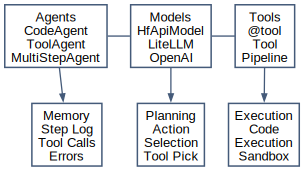
\includegraphics[keepaspectratio,alt={smolagents Architecture Diagram}]{./assets/diagram_smolagents_arch.png}}

\textbf{Agents} orchestrate the observation-thought-action loop {[}10,
12{]}.

\textbf{Models} provide the LLM interface {[}10, 12{]}.

\textbf{Tools} extend agent capabilities {[}10, 12{]}.

\textbf{Memory} tracks execution history {[}10, 12{]}.

\textbf{Planning} handles action selection {[}10, 12{]}.

\textbf{Execution} runs tool code safely {[}10, 12{]}.

\paragraph{3.3.3 Installation and Setup}\label{installation-and-setup}

\begin{Shaded}
\begin{Highlighting}[]
\CommentTok{\# Basic installation}
\ExtensionTok{pip}\NormalTok{ install smolagents}

\CommentTok{\# With Hugging Face Hub integration}
\ExtensionTok{pip}\NormalTok{ install smolagents}\PreprocessorTok{[}\SpecialStringTok{huggingface}\PreprocessorTok{]}

\CommentTok{\# With specific model providers}
\ExtensionTok{pip}\NormalTok{ install smolagents}\PreprocessorTok{[}\SpecialStringTok{litellm}\PreprocessorTok{]}      \CommentTok{\# Multi{-}provider support}
\ExtensionTok{pip}\NormalTok{ install smolagents}\PreprocessorTok{[}\SpecialStringTok{openai}\PreprocessorTok{]}       \CommentTok{\# OpenAI models}
\ExtensionTok{pip}\NormalTok{ install smolagents}\PreprocessorTok{[}\SpecialStringTok{anthropic}\PreprocessorTok{]}    \CommentTok{\# Claude models}

\CommentTok{\# Development installation}
\ExtensionTok{pip}\NormalTok{ install smolagents}\PreprocessorTok{[}\SpecialStringTok{dev}\PreprocessorTok{]}
\end{Highlighting}
\end{Shaded}

\subsubsection{3.4 CodeAgent: Code as
Action}\label{codeagent-code-as-action}

\textbf{Code labeling.} In Sections 3-6, snippets fall into two
categories: \emph{runnable examples} (intended to run with adaptation)
and \emph{pseudo-code} (architectural sketches). When helper methods or
framework internals are omitted, treat the snippet as pseudo-code.
API-facing examples were aligned to public smolagents docs/repository
references as of February 19, 2026 {[}10, 12{]}.

The flagship agent in smolagents is CodeAgent, which uses generated
Python code to invoke tools directly rather than relying only on
structured function-call objects {[}10, 12{]}.

\paragraph{3.4.1 Code as Action Paradigm}\label{code-as-action-paradigm}

Traditional agents might generate:

\begin{Shaded}
\begin{Highlighting}[]
\FunctionTok{\{}
  \DataTypeTok{"tool"}\FunctionTok{:} \StringTok{"calculator"}\FunctionTok{,}
  \DataTypeTok{"parameters"}\FunctionTok{:} \FunctionTok{\{}\DataTypeTok{"expression"}\FunctionTok{:} \StringTok{"15 * 24"}\FunctionTok{\}}
\FunctionTok{\}}
\end{Highlighting}
\end{Shaded}

CodeAgent generates:

\begin{Shaded}
\begin{Highlighting}[]
\NormalTok{calculator(expression}\OperatorTok{=}\StringTok{"15 * 24"}\NormalTok{)}
\end{Highlighting}
\end{Shaded}

In this survey\textquotesingle s implementation framing, this approach
offers several engineering advantages:

\textbf{Composability:} Multiple tools can be combined in single code
blocks:

\begin{Shaded}
\begin{Highlighting}[]
\CommentTok{\# Search for data, process it, and visualize}
\NormalTok{results }\OperatorTok{=}\NormalTok{ search(query}\OperatorTok{=}\StringTok{"Bitcoin price history"}\NormalTok{)}
\NormalTok{df }\OperatorTok{=}\NormalTok{ parse\_results(results)}
\NormalTok{chart }\OperatorTok{=}\NormalTok{ create\_chart(df, }\BuiltInTok{type}\OperatorTok{=}\StringTok{"line"}\NormalTok{)}
\NormalTok{answer }\OperatorTok{=}\NormalTok{ summarize(chart)}
\end{Highlighting}
\end{Shaded}

\textbf{Familiarity:} Python syntax is widely understood, making agent
behavior more interpretable.

\textbf{Flexibility:} Complex logic (loops, conditionals) is expressed
naturally:

\begin{Shaded}
\begin{Highlighting}[]
\ControlFlowTok{for}\NormalTok{ stock }\KeywordTok{in}\NormalTok{ [}\StringTok{"AAPL"}\NormalTok{, }\StringTok{"GOOGL"}\NormalTok{, }\StringTok{"MSFT"}\NormalTok{]:}
\NormalTok{    price }\OperatorTok{=}\NormalTok{ get\_stock\_price(stock)}
    \ControlFlowTok{if}\NormalTok{ price }\OperatorTok{\textgreater{}} \DecValTok{100}\NormalTok{:}
\NormalTok{        alert(}\SpecialStringTok{f"}\SpecialCharTok{\{}\NormalTok{stock}\SpecialCharTok{\}}\SpecialStringTok{ price alert: $}\SpecialCharTok{\{}\NormalTok{price}\SpecialCharTok{\}}\SpecialStringTok{"}\NormalTok{)}
\end{Highlighting}
\end{Shaded}

\textbf{Debugging:} Generated code can be inspected, logged, and
analyzed like any Python code.

\paragraph{3.4.2 CodeAgent
Implementation}\label{codeagent-implementation}

A minimal CodeAgent (doc-aligned pattern):

\begin{Shaded}
\begin{Highlighting}[]
\ImportTok{from}\NormalTok{ smolagents }\ImportTok{import}\NormalTok{ CodeAgent, InferenceClientModel}

\CommentTok{\# Define the agent}
\NormalTok{agent }\OperatorTok{=}\NormalTok{ CodeAgent(}
\NormalTok{    tools}\OperatorTok{=}\NormalTok{[],}
\NormalTok{    model}\OperatorTok{=}\NormalTok{InferenceClientModel(}\StringTok{"meta{-}llama/Llama{-}3.3{-}70B{-}Instruct"}\NormalTok{)}
\NormalTok{)}

\CommentTok{\# Run the agent}
\NormalTok{result }\OperatorTok{=}\NormalTok{ agent.run(}\StringTok{"What is the 15th Fibonacci number?"}\NormalTok{)}
\end{Highlighting}
\end{Shaded}

This creates an agent that can:

\begin{itemize}
\tightlist
\item
  Break down the problem into steps
\item
  Generate Python code to solve it
\item
  Execute the code in a sandboxed environment
\item
  Return the result
\end{itemize}

The agent might generate:

\begin{Shaded}
\begin{Highlighting}[]
\CommentTok{\# Calculate Fibonacci sequence}
\KeywordTok{def}\NormalTok{ fibonacci(n):}
    \ControlFlowTok{if}\NormalTok{ n }\OperatorTok{\textless{}=} \DecValTok{1}\NormalTok{:}
        \ControlFlowTok{return}\NormalTok{ n}
\NormalTok{    a, b }\OperatorTok{=} \DecValTok{0}\NormalTok{, }\DecValTok{1}
    \ControlFlowTok{for}\NormalTok{ \_ }\KeywordTok{in} \BuiltInTok{range}\NormalTok{(}\DecValTok{2}\NormalTok{, n }\OperatorTok{+} \DecValTok{1}\NormalTok{):}
\NormalTok{        a, b }\OperatorTok{=}\NormalTok{ b, a }\OperatorTok{+}\NormalTok{ b}
    \ControlFlowTok{return}\NormalTok{ b}

\NormalTok{result }\OperatorTok{=}\NormalTok{ fibonacci(}\DecValTok{15}\NormalTok{)}
\BuiltInTok{print}\NormalTok{(result)}
\end{Highlighting}
\end{Shaded}

\paragraph{3.4.3 Configuration and
Customization}\label{configuration-and-customization}

CodeAgent configuration options in current docs include model/tool
binding, step limits, optional planning, authorized imports, grammar,
and executor settings {[}10, 12{]}:

\begin{Shaded}
\begin{Highlighting}[]
\ImportTok{from}\NormalTok{ smolagents }\ImportTok{import}\NormalTok{ CodeAgent, InferenceClientModel}
\ImportTok{from}\NormalTok{ smolagents.default\_tools }\ImportTok{import}\NormalTok{ DuckDuckGoSearchTool}

\NormalTok{agent }\OperatorTok{=}\NormalTok{ CodeAgent(}
\NormalTok{    tools}\OperatorTok{=}\NormalTok{[DuckDuckGoSearchTool()],}
\NormalTok{    model}\OperatorTok{=}\NormalTok{InferenceClientModel(}\StringTok{"meta{-}llama/Llama{-}3.3{-}70B{-}Instruct"}\NormalTok{),}
\NormalTok{    max\_steps}\OperatorTok{=}\DecValTok{10}\NormalTok{,}
\NormalTok{    planning\_interval}\OperatorTok{=}\DecValTok{3}\NormalTok{,}
\NormalTok{    additional\_authorized\_imports}\OperatorTok{=}\NormalTok{[}\StringTok{"math"}\NormalTok{, }\StringTok{"random"}\NormalTok{],}
\NormalTok{    grammar}\OperatorTok{=}\VariableTok{None}\NormalTok{,}
\NormalTok{    executor\_type}\OperatorTok{=}\StringTok{"local"}\NormalTok{,}
\NormalTok{    executor\_kwargs}\OperatorTok{=}\VariableTok{None}
\NormalTok{)}
\end{Highlighting}
\end{Shaded}

\subsubsection{3.5 MultiStepAgent: Managing Complex
Workflows}\label{multistepagent-managing-complex-workflows}

For tasks requiring multiple distinct phases or extended reasoning,
smolagents provides MultiStepAgent with explicit planning/state patterns
{[}10, 12{]}.

\paragraph{3.5.1 Multi-Step Architecture}\label{multi-step-architecture}

MultiStepAgent maintains richer state across execution:

\pandocbounded{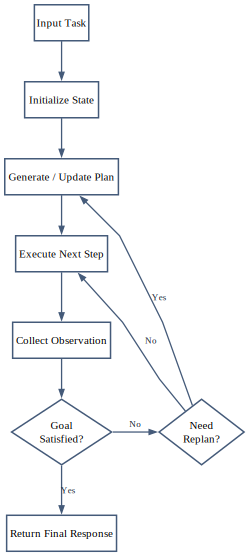
\includegraphics[keepaspectratio,alt={MultiStepAgent State Diagram}]{./assets/diagram_multistep_state.png}}

\paragraph{3.5.2 Planning Capabilities}\label{planning-capabilities}

MultiStepAgent can create and execute plans:

\begin{Shaded}
\begin{Highlighting}[]
\ImportTok{from}\NormalTok{ smolagents }\ImportTok{import}\NormalTok{ MultiStepAgent, InferenceClientModel}

\NormalTok{agent }\OperatorTok{=}\NormalTok{ MultiStepAgent(}
\NormalTok{    tools}\OperatorTok{=}\NormalTok{[search, calculator, summarize],}
\NormalTok{    model}\OperatorTok{=}\NormalTok{InferenceClientModel(}\StringTok{"Qwen/Qwen2.5{-}Coder{-}32B{-}Instruct"}\NormalTok{),}
\NormalTok{    planning\_interval}\OperatorTok{=}\DecValTok{2}  \CommentTok{\# Re{-}plan every 2 steps}
\NormalTok{)}

\NormalTok{result }\OperatorTok{=}\NormalTok{ agent.run(}\StringTok{"""}
\StringTok{    Analyze the impact of recent AI regulations on tech stocks. }
\StringTok{    Search for news, gather price data for major companies, }
\StringTok{    and summarize the findings.}
\StringTok{"""}\NormalTok{)}
\end{Highlighting}
\end{Shaded}

The agent might:

\begin{enumerate}
\tightlist
\item
  Plan: "1. Search AI regulation news, 2. Get stock prices, 3. Analyze
  correlation, 4. Summarize"
\item
  Execute plan step by step
\item
  Re-plan if initial approach proves insufficient
\item
  Maintain context across all steps
\end{enumerate}

\paragraph{3.5.3 Error Handling and
Recovery}\label{error-handling-and-recovery}

Error handling is typically implemented at orchestration level around
agent execution (pseudo-code sketch):

\begin{Shaded}
\begin{Highlighting}[]
\ImportTok{from}\NormalTok{ smolagents }\ImportTok{import}\NormalTok{ MultiStepAgent}

\NormalTok{agent }\OperatorTok{=}\NormalTok{ MultiStepAgent(}
\NormalTok{    tools}\OperatorTok{=}\NormalTok{tools,}
\NormalTok{    model}\OperatorTok{=}\NormalTok{model,}
\NormalTok{    max\_steps}\OperatorTok{=}\DecValTok{20}\NormalTok{,}
\NormalTok{    planning\_interval}\OperatorTok{=}\DecValTok{3}
\NormalTok{)}

\CommentTok{\# Pseudo{-}code orchestration pattern}
\ControlFlowTok{for}\NormalTok{ attempt }\KeywordTok{in} \BuiltInTok{range}\NormalTok{(}\DecValTok{3}\NormalTok{):}
    \ControlFlowTok{try}\NormalTok{:}
\NormalTok{        result }\OperatorTok{=}\NormalTok{ agent.run(task)}
        \ControlFlowTok{break}
    \ControlFlowTok{except} \PreprocessorTok{Exception} \ImportTok{as}\NormalTok{ err:}
\NormalTok{        log\_error(err)}
\NormalTok{        task }\OperatorTok{=}\NormalTok{ add\_recovery\_context(task, err)}
\CommentTok{\# Report final outcome or propagate terminal error}
\end{Highlighting}
\end{Shaded}

\subsubsection{3.6 The Tool Ecosystem}\label{the-tool-ecosystem}

Tools extend agent capabilities beyond language generation, enabling
interaction with external systems, data sources, and services {[}6,
10{]}.

\paragraph{3.6.1 Built-in Tools}\label{built-in-tools}

smolagents provides default tool integrations (examples below are
doc-aligned) {[}10, 12{]}:

\textbf{Search and browsing tools:}

\begin{Shaded}
\begin{Highlighting}[]
\ImportTok{from}\NormalTok{ smolagents.default\_tools }\ImportTok{import}\NormalTok{ (}
\NormalTok{    DuckDuckGoSearchTool,}
\NormalTok{    WikipediaSearchTool,}
\NormalTok{    VisitWebpageTool,}
\NormalTok{)}

\NormalTok{search\_tool }\OperatorTok{=}\NormalTok{ DuckDuckGoSearchTool()}
\NormalTok{wiki\_tool }\OperatorTok{=}\NormalTok{ WikipediaSearchTool()}
\NormalTok{visit\_tool }\OperatorTok{=}\NormalTok{ VisitWebpageTool()}
\end{Highlighting}
\end{Shaded}

\textbf{Python execution tool:}

\begin{Shaded}
\begin{Highlighting}[]
\ImportTok{from}\NormalTok{ smolagents }\ImportTok{import}\NormalTok{ PythonInterpreterTool}

\NormalTok{python\_tool }\OperatorTok{=}\NormalTok{ PythonInterpreterTool()}
\NormalTok{result }\OperatorTok{=}\NormalTok{ python\_tool(}\StringTok{"sum(range(100))"}\NormalTok{)}
\end{Highlighting}
\end{Shaded}

\paragraph{3.6.2 Custom Tool Definition}\label{custom-tool-definition}

Tools are defined using Python decorators {[}10, 12{]}:

\begin{Shaded}
\begin{Highlighting}[]
\ImportTok{from}\NormalTok{ smolagents }\ImportTok{import}\NormalTok{ tool}
\ImportTok{from}\NormalTok{ typing }\ImportTok{import}\NormalTok{ Optional}

\AttributeTok{@tool}
\KeywordTok{def}\NormalTok{ fetch\_stock\_price(}
\NormalTok{    ticker: }\BuiltInTok{str}\NormalTok{,}
\NormalTok{    date: Optional[}\BuiltInTok{str}\NormalTok{] }\OperatorTok{=} \VariableTok{None}
\NormalTok{) }\OperatorTok{{-}\textgreater{}} \BuiltInTok{str}\NormalTok{:}
    \CommentTok{"""}
\CommentTok{    Fetch the current or historical stock price for a given ticker symbol.}
\CommentTok{    }
\CommentTok{    Args:}
\CommentTok{        ticker: The stock ticker symbol (e.g., \textquotesingle{}AAPL\textquotesingle{}, \textquotesingle{}GOOGL\textquotesingle{})}
\CommentTok{        date: Optional date in YYYY{-}MM{-}DD format for historical data.}
\CommentTok{              If not provided, returns current price.}
\CommentTok{    }
\CommentTok{    Returns:}
\CommentTok{        The stock price as a string with currency.}
\CommentTok{    """}
    \CommentTok{\# Implementation would call financial API}
    \CommentTok{\# For demonstration:}
    \ControlFlowTok{if}\NormalTok{ ticker }\OperatorTok{==} \StringTok{"AAPL"}\NormalTok{:}
        \ControlFlowTok{return} \StringTok{"$175.50"}
    \ControlFlowTok{return} \StringTok{"Price data not available"}
\end{Highlighting}
\end{Shaded}

The \texttt{@tool} decorator (conceptually):

\begin{itemize}
\tightlist
\item
  Parses the docstring for tool description
\item
  Extracts type hints for parameter validation
\item
  Registers the function as available to agents
\item
  Generates tool schemas for LLM function calling
\end{itemize}

\paragraph{3.6.3 Tool Integration
Patterns}\label{tool-integration-patterns}

Tools can be combined in sophisticated ways:

\textbf{Chained Tools:}

\begin{Shaded}
\begin{Highlighting}[]
\AttributeTok{@tool}
\KeywordTok{def}\NormalTok{ analyze\_website(url: }\BuiltInTok{str}\NormalTok{) }\OperatorTok{{-}\textgreater{}} \BuiltInTok{str}\NormalTok{:}
    \CommentTok{"""Analyze a website and return key information."""}
    \CommentTok{\# Step 1: Fetch content}
\NormalTok{    content }\OperatorTok{=}\NormalTok{ fetch\_url(url)}
    
    \CommentTok{\# Step 2: Extract text}
\NormalTok{    text }\OperatorTok{=}\NormalTok{ extract\_text(content)}
    
    \CommentTok{\# Step 3: Summarize}
\NormalTok{    summary }\OperatorTok{=}\NormalTok{ summarize(text)}
    
    \ControlFlowTok{return}\NormalTok{ summary}
\end{Highlighting}
\end{Shaded}

\textbf{Conditional Tools:}

\begin{Shaded}
\begin{Highlighting}[]
\AttributeTok{@tool}
\KeywordTok{def}\NormalTok{ smart\_search(query: }\BuiltInTok{str}\NormalTok{, require\_recent: }\BuiltInTok{bool} \OperatorTok{=} \VariableTok{False}\NormalTok{) }\OperatorTok{{-}\textgreater{}} \BuiltInTok{str}\NormalTok{:}
    \CommentTok{"""Search with conditional logic."""}
    \ControlFlowTok{if}\NormalTok{ require\_recent:}
        \ControlFlowTok{return}\NormalTok{ news\_search(query, days}\OperatorTok{=}\DecValTok{7}\NormalTok{)}
    \ControlFlowTok{else}\NormalTok{:}
        \ControlFlowTok{return}\NormalTok{ web\_search(query)}
\end{Highlighting}
\end{Shaded}

\textbf{Stateful Tools:}

\begin{Shaded}
\begin{Highlighting}[]
\KeywordTok{class}\NormalTok{ DatabaseTool:}
    \KeywordTok{def} \FunctionTok{\_\_init\_\_}\NormalTok{(}\VariableTok{self}\NormalTok{):}
        \VariableTok{self}\NormalTok{.connection }\OperatorTok{=} \VariableTok{None}
    
    \AttributeTok{@tool}
    \KeywordTok{def}\NormalTok{ query(}\VariableTok{self}\NormalTok{, sql: }\BuiltInTok{str}\NormalTok{) }\OperatorTok{{-}\textgreater{}} \BuiltInTok{str}\NormalTok{:}
        \CommentTok{"""Execute SQL query on connected database."""}
        \ControlFlowTok{if} \KeywordTok{not} \VariableTok{self}\NormalTok{.connection:}
            \VariableTok{self}\NormalTok{.}\ExtensionTok{connect}\NormalTok{()}
        \ControlFlowTok{return} \VariableTok{self}\NormalTok{.connection.execute(sql).fetchall()}
    
    \AttributeTok{@tool}
    \KeywordTok{def}\NormalTok{ schema(}\VariableTok{self}\NormalTok{) }\OperatorTok{{-}\textgreater{}} \BuiltInTok{str}\NormalTok{:}
        \CommentTok{"""Return database schema."""}
        \ControlFlowTok{return} \VariableTok{self}\NormalTok{.get\_schema()}
\end{Highlighting}
\end{Shaded}

\paragraph{3.6.4 Tool Schemas and
Validation}\label{tool-schemas-and-validation}

smolagents supports tool schema generation/serialization for callable
interfaces {[}10, 12{]}:

\begin{Shaded}
\begin{Highlighting}[]
\CommentTok{\# For the fetch\_stock\_price tool above, the schema is:}
\NormalTok{\{}
    \StringTok{"name"}\NormalTok{: }\StringTok{"fetch\_stock\_price"}\NormalTok{,}
    \StringTok{"description"}\NormalTok{: }\StringTok{"Fetch the current or historical stock price..."}\NormalTok{,}
    \StringTok{"parameters"}\NormalTok{: \{}
        \StringTok{"type"}\NormalTok{: }\StringTok{"object"}\NormalTok{,}
        \StringTok{"properties"}\NormalTok{: \{}
            \StringTok{"ticker"}\NormalTok{: \{}
                \StringTok{"type"}\NormalTok{: }\StringTok{"string"}\NormalTok{,}
                \StringTok{"description"}\NormalTok{: }\StringTok{"The stock ticker symbol..."}
\NormalTok{            \},}
            \StringTok{"date"}\NormalTok{: \{}
                \StringTok{"type"}\NormalTok{: }\StringTok{"string"}\NormalTok{,}
                \StringTok{"description"}\NormalTok{: }\StringTok{"Optional date in YYYY{-}MM{-}DD format..."}\NormalTok{,}
                \StringTok{"nullable"}\NormalTok{: true}
\NormalTok{            \}}
\NormalTok{        \},}
        \StringTok{"required"}\NormalTok{: [}\StringTok{"ticker"}\NormalTok{]}
\NormalTok{    \}}
\NormalTok{\}}
\end{Highlighting}
\end{Shaded}

This schema enables:

\begin{itemize}
\tightlist
\item
  \textbf{LLM Understanding:} The model knows available tools and their
  parameters
\item
  \textbf{Validation:} Inputs are checked against types before execution
\item
  \textbf{Documentation:} Clear descriptions guide model usage
\item
  \textbf{Interoperability:} Standard format works across frameworks
\end{itemize}

\paragraph{3.6.5 The Tool-Augmented LLM
Pattern}\label{the-tool-augmented-llm-pattern}

The integration of tools with LLMs follows a recurring pattern in agent
frameworks {[}6, 10{]}:

\pandocbounded{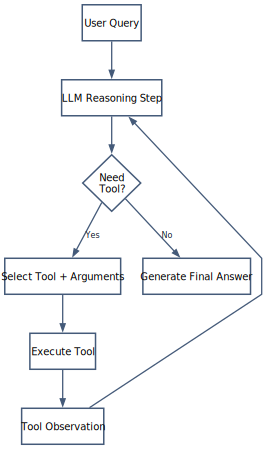
\includegraphics[keepaspectratio,alt={Tool-Augmented LLM Flow Diagram}]{./assets/diagram_tool_flow.png}}

This pattern, associated with reasoning-action workflows such as ReAct
and related agent frameworks, enables LLMs to {[}6, 10{]}:

\begin{itemize}
\tightlist
\item
  Access information beyond their training data
\item
  Perform computations beyond their parametric capacity
\item
  Interact with external systems and APIs
\item
  Verify facts through live data sources
\end{itemize}

The smolagents implementation provides this pattern through lightweight
framework abstractions {[}10, 12{]}.

\paragraph{3.6.6 Tool Security and
Sandboxing}\label{tool-security-and-sandboxing}

Security is critical when agents execute generated code. Current
smolagents patterns center on executor selection plus environment
controls {[}10, 12{]}:

\textbf{Executor selection:}

\begin{Shaded}
\begin{Highlighting}[]
\ImportTok{from}\NormalTok{ smolagents }\ImportTok{import}\NormalTok{ CodeAgent, InferenceClientModel}

\NormalTok{agent }\OperatorTok{=}\NormalTok{ CodeAgent(}
\NormalTok{    tools}\OperatorTok{=}\NormalTok{tools,}
\NormalTok{    model}\OperatorTok{=}\NormalTok{InferenceClientModel(}\StringTok{"meta{-}llama/Llama{-}3.3{-}70B{-}Instruct"}\NormalTok{),}
\NormalTok{    additional\_authorized\_imports}\OperatorTok{=}\NormalTok{[}\StringTok{"math"}\NormalTok{, }\StringTok{"datetime"}\NormalTok{],}
\NormalTok{    executor\_type}\OperatorTok{=}\StringTok{"docker"}\NormalTok{,   }\CommentTok{\# examples: local, docker, e2b, modal, wasm}
\NormalTok{    executor\_kwargs}\OperatorTok{=}\NormalTok{\{...\},    }\CommentTok{\# backend{-}specific settings}
\NormalTok{)}
\end{Highlighting}
\end{Shaded}

Network policy, CPU/memory limits, and host restrictions are typically
enforced by the selected execution backend (container/runtime platform),
not by a single universal smolagents runtime API. These controls support
safer deployment patterns, but production safety still depends on
environment-specific hardening and policy review {[}10, 12{]}.

\subsubsection{3.7 Deployment and
Production}\label{deployment-and-production}

\paragraph{3.7.1 Deployment Patterns}\label{deployment-patterns}

\textbf{Local Deployment:}

\begin{Shaded}
\begin{Highlighting}[]
\CommentTok{\# FastAPI wrapper for local serving}
\ImportTok{from}\NormalTok{ fastapi }\ImportTok{import}\NormalTok{ FastAPI}
\ImportTok{from}\NormalTok{ smolagents }\ImportTok{import}\NormalTok{ CodeAgent}

\NormalTok{app }\OperatorTok{=}\NormalTok{ FastAPI()}
\NormalTok{agent }\OperatorTok{=}\NormalTok{ CodeAgent(tools}\OperatorTok{=}\NormalTok{[...], model}\OperatorTok{=}\NormalTok{model)}

\AttributeTok{@app.post}\NormalTok{(}\StringTok{"/chat"}\NormalTok{)}
\ControlFlowTok{async} \KeywordTok{def}\NormalTok{ chat(request: ChatRequest):}
\NormalTok{    response }\OperatorTok{=}\NormalTok{ agent.run(request.message)}
    \ControlFlowTok{return}\NormalTok{ \{}\StringTok{"response"}\NormalTok{: response\}}
\end{Highlighting}
\end{Shaded}

\textbf{Containerized Deployment:}

\begin{Shaded}
\begin{Highlighting}[]
\KeywordTok{FROM}\NormalTok{ python:3.11{-}slim}
\KeywordTok{WORKDIR}\NormalTok{ /app}
\KeywordTok{COPY}\NormalTok{ requirements.txt .}
\KeywordTok{RUN} \ExtensionTok{pip}\NormalTok{ install }\AttributeTok{{-}r}\NormalTok{ requirements.txt}
\KeywordTok{COPY}\NormalTok{ . .}
\KeywordTok{EXPOSE}\NormalTok{ 8000}
\KeywordTok{CMD}\NormalTok{ [}\StringTok{"uvicorn"}\NormalTok{, }\StringTok{"main:app"}\NormalTok{, }\StringTok{"{-}{-}host"}\NormalTok{, }\StringTok{"0.0.0.0"}\NormalTok{, }\StringTok{"{-}{-}port"}\NormalTok{, }\StringTok{"8000"}\NormalTok{]}
\end{Highlighting}
\end{Shaded}

\paragraph{3.7.2 Monitoring and
Observability}\label{monitoring-and-observability}

\begin{Shaded}
\begin{Highlighting}[]
\CommentTok{\# Instrumented agent with tracing}
\ImportTok{from}\NormalTok{ smolagents }\ImportTok{import}\NormalTok{ CodeAgent}
\ImportTok{import}\NormalTok{ opentelemetry}

\KeywordTok{class}\NormalTok{ InstrumentedAgent(CodeAgent):}
    \KeywordTok{def}\NormalTok{ run(}\VariableTok{self}\NormalTok{, task, }\OperatorTok{**}\NormalTok{kwargs):}
        \ControlFlowTok{with}\NormalTok{ tracer.start\_as\_current\_span(}\StringTok{"agent\_run"}\NormalTok{) }\ImportTok{as}\NormalTok{ span:}
\NormalTok{            span.set\_attribute(}\StringTok{"task"}\NormalTok{, task)}
\NormalTok{            start\_time }\OperatorTok{=}\NormalTok{ time.time()}
            
\NormalTok{            result }\OperatorTok{=} \BuiltInTok{super}\NormalTok{().run(task, }\OperatorTok{**}\NormalTok{kwargs)}
            
\NormalTok{            span.set\_attribute(}\StringTok{"duration"}\NormalTok{, time.time() }\OperatorTok{{-}}\NormalTok{ start\_time)}
\NormalTok{            span.set\_attribute(}\StringTok{"steps"}\NormalTok{, }\BuiltInTok{len}\NormalTok{(}\VariableTok{self}\NormalTok{.memory))}
\NormalTok{            span.set\_attribute(}\StringTok{"tools\_used"}\NormalTok{, }\BuiltInTok{list}\NormalTok{(}\VariableTok{self}\NormalTok{.tools.keys()))}
            
            \ControlFlowTok{return}\NormalTok{ result}
\end{Highlighting}
\end{Shaded}

\begin{center}\rule{0.5\linewidth}{0.5pt}\end{center}

\subsection{4. Synthesis: Enhancing Hugging Face Agents with Tree of
Thoughts}\label{synthesis-enhancing-hugging-face-agents-with-tree-of-thoughts}

\subsubsection{4.1 The Convergence of Reasoning and
Action}\label{the-convergence-of-reasoning-and-action}

This section describes a design synthesis: combining Tree of Thoughts
with Hugging Face agents. While Hugging Face agents provide strong
tooling interfaces, many workflows still use linear reasoning traces. A
ToT-style planner can introduce {[}1, 10, 12{]}:

\begin{enumerate}
\tightlist
\item
  \textbf{Explore multiple solution strategies} before committing to
  actions
\item
  \textbf{Evaluate tool sequences} before execution
\item
  \textbf{Backtrack from unsuccessful tool calls}
\item
  \textbf{Plan multi-step operations} with lookahead evaluation
\item
  \textbf{Recover from errors} through alternative reasoning paths
\end{enumerate}

\subsubsection{4.2 Architectural
Integration}\label{architectural-integration}

\paragraph{4.2.1 ToT-Enhanced Agent
Architecture}\label{tot-enhanced-agent-architecture}

\pandocbounded{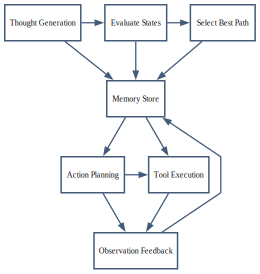
\includegraphics[keepaspectratio,alt={ToT-Enhanced Agent Architecture Diagram}]{./assets/diagram_tot_agent.png}}

\paragraph{4.2.2 Implementation Sketch (Pseudo-code): ToT Code
Agent}\label{implementation-sketch-pseudo-code-tot-code-agent}

\begin{Shaded}
\begin{Highlighting}[]
\ImportTok{from}\NormalTok{ smolagents }\ImportTok{import}\NormalTok{ CodeAgent, InferenceClientModel}
\ImportTok{from}\NormalTok{ typing }\ImportTok{import}\NormalTok{ List, Dict, Any}
\ImportTok{import}\NormalTok{ heapq}

\KeywordTok{class}\NormalTok{ TreeOfThoughtsCodeAgent(CodeAgent):}
    \CommentTok{"""Agent that uses Tree of Thoughts for planning before execution."""}
    
    \KeywordTok{def} \FunctionTok{\_\_init\_\_}\NormalTok{(}\VariableTok{self}\NormalTok{, }\OperatorTok{*}\NormalTok{args, beam\_width}\OperatorTok{=}\DecValTok{3}\NormalTok{, max\_depth}\OperatorTok{=}\DecValTok{5}\NormalTok{, }\OperatorTok{**}\NormalTok{kwargs):}
        \BuiltInTok{super}\NormalTok{().}\FunctionTok{\_\_init\_\_}\NormalTok{(}\OperatorTok{*}\NormalTok{args, }\OperatorTok{**}\NormalTok{kwargs)}
        \VariableTok{self}\NormalTok{.beam\_width }\OperatorTok{=}\NormalTok{ beam\_width}
        \VariableTok{self}\NormalTok{.max\_depth }\OperatorTok{=}\NormalTok{ max\_depth}
    
    \KeywordTok{def}\NormalTok{ generate\_thoughts(}\VariableTok{self}\NormalTok{, task: }\BuiltInTok{str}\NormalTok{, current\_state: }\BuiltInTok{str}\NormalTok{, k: }\BuiltInTok{int}\NormalTok{) }\OperatorTok{{-}\textgreater{}}\NormalTok{ List[}\BuiltInTok{str}\NormalTok{]:}
        \CommentTok{"""Generate k candidate next steps."""}
\NormalTok{        prompt }\OperatorTok{=} \SpecialStringTok{f"""}
\SpecialStringTok{Given the task: }\SpecialCharTok{\{}\NormalTok{task}\SpecialCharTok{\}}
\SpecialStringTok{And current progress: }\SpecialCharTok{\{}\NormalTok{current\_state}\SpecialCharTok{\}}

\SpecialStringTok{Generate }\SpecialCharTok{\{}\NormalTok{k}\SpecialCharTok{\}}\SpecialStringTok{ different possible next actions. Each action should be }
\SpecialStringTok{a concrete step toward solving the problem. Be diverse in your approaches.}

\SpecialStringTok{Format as a numbered list:}
\SpecialStringTok{1. [First approach]}
\SpecialStringTok{2. [Second approach]}
\SpecialStringTok{...}
\SpecialStringTok{"""}
\NormalTok{        response }\OperatorTok{=} \VariableTok{self}\NormalTok{.model.generate(prompt)}
\NormalTok{        thoughts }\OperatorTok{=} \VariableTok{self}\NormalTok{.\_parse\_numbered\_list(response, k)}
        \ControlFlowTok{return}\NormalTok{ thoughts}
    
    \KeywordTok{def}\NormalTok{ evaluate\_thought(}\VariableTok{self}\NormalTok{, task: }\BuiltInTok{str}\NormalTok{, thought: }\BuiltInTok{str}\NormalTok{, history: List[}\BuiltInTok{str}\NormalTok{]) }\OperatorTok{{-}\textgreater{}} \BuiltInTok{float}\NormalTok{:}
        \CommentTok{"""Score a thought\textquotesingle{}s promise (0{-}10)."""}
\NormalTok{        prompt }\OperatorTok{=} \SpecialStringTok{f"""}
\SpecialStringTok{Task: }\SpecialCharTok{\{}\NormalTok{task}\SpecialCharTok{\}}
\SpecialStringTok{Proposed action: }\SpecialCharTok{\{}\NormalTok{thought}\SpecialCharTok{\}}
\SpecialStringTok{History so far: }\SpecialCharTok{\{}\StringTok{\textquotesingle{} {-}\textgreater{} \textquotesingle{}}\SpecialCharTok{.}\NormalTok{join(history)}\SpecialCharTok{\}}

\SpecialStringTok{Rate how promising this action is on a scale of 0{-}10:}
\SpecialStringTok{{-} 0{-}3: Likely incorrect or counterproductive}
\SpecialStringTok{{-} 4{-}6: Might help but uncertain}
\SpecialStringTok{{-} 7{-}10: Clearly advances toward solution}

\SpecialStringTok{Return ONLY a number between 0 and 10.}
\SpecialStringTok{"""}
        \ControlFlowTok{try}\NormalTok{:}
\NormalTok{            score\_text }\OperatorTok{=} \VariableTok{self}\NormalTok{.model.generate(prompt).strip()}
            \ControlFlowTok{return} \BuiltInTok{float}\NormalTok{(score\_text.split()[}\DecValTok{0}\NormalTok{])}
        \ControlFlowTok{except}\NormalTok{:}
            \ControlFlowTok{return} \FloatTok{5.0}  \CommentTok{\# Default to uncertain}
    
    \KeywordTok{def}\NormalTok{ beam\_search\_planning(}\VariableTok{self}\NormalTok{, task: }\BuiltInTok{str}\NormalTok{) }\OperatorTok{{-}\textgreater{}}\NormalTok{ List[}\BuiltInTok{str}\NormalTok{]:}
        \CommentTok{"""Use beam search to find best action sequence."""}
        \CommentTok{\# Initialize: [(score, actions, state)]}
\NormalTok{        beams }\OperatorTok{=}\NormalTok{ [(}\FloatTok{0.0}\NormalTok{, [], }\StringTok{"Initial state"}\NormalTok{)]}
        
        \ControlFlowTok{for}\NormalTok{ depth }\KeywordTok{in} \BuiltInTok{range}\NormalTok{(}\VariableTok{self}\NormalTok{.max\_depth):}
\NormalTok{            candidates }\OperatorTok{=}\NormalTok{ []}
            
            \ControlFlowTok{for}\NormalTok{ score, actions, state }\KeywordTok{in}\NormalTok{ beams:}
                \CommentTok{\# Generate next thoughts}
\NormalTok{                thoughts }\OperatorTok{=} \VariableTok{self}\NormalTok{.generate\_thoughts(task, state, }\VariableTok{self}\NormalTok{.beam\_width)}
                
                \ControlFlowTok{for}\NormalTok{ thought }\KeywordTok{in}\NormalTok{ thoughts:}
                    \CommentTok{\# Simulate action (lightweight evaluation)}
\NormalTok{                    new\_state }\OperatorTok{=} \SpecialStringTok{f"}\SpecialCharTok{\{}\NormalTok{state}\SpecialCharTok{\}}\SpecialStringTok{ {-}\textgreater{} }\SpecialCharTok{\{}\NormalTok{thought}\SpecialCharTok{\}}\SpecialStringTok{"}
\NormalTok{                    new\_actions }\OperatorTok{=}\NormalTok{ actions }\OperatorTok{+}\NormalTok{ [thought]}
                    
                    \CommentTok{\# Evaluate}
\NormalTok{                    value }\OperatorTok{=} \VariableTok{self}\NormalTok{.evaluate\_thought(task, thought, actions)}
\NormalTok{                    total\_score }\OperatorTok{=}\NormalTok{ score }\OperatorTok{+}\NormalTok{ value}
                    
\NormalTok{                    candidates.append((total\_score, new\_actions, new\_state))}
            
            \CommentTok{\# Keep top beams}
\NormalTok{            beams }\OperatorTok{=}\NormalTok{ heapq.nlargest(}\VariableTok{self}\NormalTok{.beam\_width, candidates, key}\OperatorTok{=}\KeywordTok{lambda}\NormalTok{ x: x[}\DecValTok{0}\NormalTok{])}
        
        \CommentTok{\# Return best action sequence}
        \ControlFlowTok{return}\NormalTok{ beams[}\DecValTok{0}\NormalTok{][}\DecValTok{1}\NormalTok{] }\ControlFlowTok{if}\NormalTok{ beams }\ControlFlowTok{else}\NormalTok{ []}
    
    \KeywordTok{def}\NormalTok{ run(}\VariableTok{self}\NormalTok{, task: }\BuiltInTok{str}\NormalTok{, }\OperatorTok{**}\NormalTok{kwargs):}
        \CommentTok{"""Execute with ToT planning."""}
        \CommentTok{\# Phase 1: Plan with ToT}
        \BuiltInTok{print}\NormalTok{(}\StringTok{"Planning with Tree of Thoughts..."}\NormalTok{)}
\NormalTok{        action\_plan }\OperatorTok{=} \VariableTok{self}\NormalTok{.beam\_search\_planning(task)}
        \BuiltInTok{print}\NormalTok{(}\SpecialStringTok{f"Selected plan: }\SpecialCharTok{\{}\NormalTok{action\_plan}\SpecialCharTok{\}}\SpecialStringTok{"}\NormalTok{)}
        
        \CommentTok{\# Phase 2: Execute planned actions}
        \CommentTok{\# (simplified {-} full implementation would integrate with CodeAgent execution)}
        \ControlFlowTok{return} \VariableTok{self}\NormalTok{.execute\_plan(task, action\_plan)}

\CommentTok{\# Usage}
\NormalTok{agent }\OperatorTok{=}\NormalTok{ TreeOfThoughtsCodeAgent(}
\NormalTok{    tools}\OperatorTok{=}\NormalTok{[search\_tool, calculator\_tool],}
\NormalTok{    model}\OperatorTok{=}\NormalTok{InferenceClientModel(}\StringTok{"meta{-}llama/Llama{-}3.3{-}70B{-}Instruct"}\NormalTok{),}
\NormalTok{    beam\_width}\OperatorTok{=}\DecValTok{3}\NormalTok{,}
\NormalTok{    max\_depth}\OperatorTok{=}\DecValTok{4}
\NormalTok{)}

\NormalTok{result }\OperatorTok{=}\NormalTok{ agent.run(}\StringTok{"""}
\StringTok{Analyze the economic impact of AI on job markets. }
\StringTok{Search for recent data, calculate key statistics, }
\StringTok{and summarize the findings.}
\StringTok{"""}\NormalTok{)}
\end{Highlighting}
\end{Shaded}

\subsubsection{4.3 Design-Level Benefits
(Hypothesized)}\label{design-level-benefits-hypothesized}

\paragraph{4.3.1 Improved Tool Selection}\label{improved-tool-selection}

\textbf{Problem:} Agents often select suboptimal tools or sequences.

\textbf{ToT Solution:} Explore multiple tool sequences before execution.

\begin{Shaded}
\begin{Highlighting}[]
\CommentTok{\# Traditional approach}
\KeywordTok{def}\NormalTok{ traditional\_agent(task):}
\NormalTok{    thought }\OperatorTok{=}\NormalTok{ model.generate(}\SpecialStringTok{f"What tool for: }\SpecialCharTok{\{}\NormalTok{task}\SpecialCharTok{\}}\SpecialStringTok{?"}\NormalTok{)}
\NormalTok{    tool\_call }\OperatorTok{=}\NormalTok{ parse\_tool(thought)}
\NormalTok{    result }\OperatorTok{=}\NormalTok{ execute(tool\_call)}
    \CommentTok{\# No alternative considered}

\CommentTok{\# ToT{-}enhanced approach}
\KeywordTok{def}\NormalTok{ tot\_agent(task):}
\NormalTok{    candidates }\OperatorTok{=}\NormalTok{ [}
        \StringTok{"Use web\_search then summarize"}\NormalTok{,}
        \StringTok{"Use calculator then web\_search"}\NormalTok{,}
        \StringTok{"Use knowledge\_base directly"}
\NormalTok{    ]}
    
    \CommentTok{\# Simulate and evaluate each}
\NormalTok{    scores }\OperatorTok{=}\NormalTok{ [evaluate\_path(task, path) }\ControlFlowTok{for}\NormalTok{ path }\KeywordTok{in}\NormalTok{ candidates]}
\NormalTok{    best }\OperatorTok{=}\NormalTok{ candidates[argmax(scores)]}
    
    \ControlFlowTok{return}\NormalTok{ execute(best)}
\end{Highlighting}
\end{Shaded}

\textbf{Example - Complex Query:}

\begin{Shaded}
\begin{Highlighting}[]
\NormalTok{Task: "Compare Tesla and BYD stock performance over the last year"}

\NormalTok{ToT Exploration:}
\NormalTok{|-- Path A: Search for both, then compare}
\NormalTok{|   |-- Step 1: search("Tesla stock 2024")}
\NormalTok{|   |-- Step 2: search("BYD stock 2024")}
\NormalTok{|   `-- Step 3: calculate(comparison\_metrics)}
\NormalTok{|   `-- Heuristic rating: medium (detailed but may miss real{-}time data)}
\NormalTok{|}
\NormalTok{|-- Path B: Use stock API directly}
\NormalTok{|   |-- Step 1: stock\_api("TSLA", period="1y")}
\NormalTok{|   |-- Step 2: stock\_api("BYD", period="1y")}
\NormalTok{|   `-- Step 3: calculate\_performance\_comparison}
\NormalTok{|   `-- Heuristic rating: high (precise data, structured output)}
\NormalTok{|}
\NormalTok{`-- Path C: Search for analysis articles}
\NormalTok{    `-- Heuristic rating: low (subjective, may be outdated)}

\NormalTok{Selected: Path B for accuracy and reliability}
\end{Highlighting}
\end{Shaded}

\paragraph{4.3.2 Error Recovery and
Backtracking}\label{error-recovery-and-backtracking}

\textbf{Problem:} When tool calls fail, agents often get stuck or
produce incorrect results.

\textbf{ToT Solution:} Maintain alternative paths for backtracking.

\begin{Shaded}
\begin{Highlighting}[]
\KeywordTok{class}\NormalTok{ RecoverableAgent(TreeOfThoughtsCodeAgent):}
    \KeywordTok{def}\NormalTok{ execute\_with\_recovery(}\VariableTok{self}\NormalTok{, action\_plan):}
        \ControlFlowTok{for}\NormalTok{ i, action }\KeywordTok{in} \BuiltInTok{enumerate}\NormalTok{(action\_plan):}
            \ControlFlowTok{try}\NormalTok{:}
\NormalTok{                result }\OperatorTok{=} \VariableTok{self}\NormalTok{.execute\_action(action)}
                \ControlFlowTok{if} \VariableTok{self}\NormalTok{.verify\_result(result):}
                    \ControlFlowTok{continue}
                \ControlFlowTok{else}\NormalTok{:}
                    \CommentTok{\# Result suspicious, try alternative}
\NormalTok{                    alternatives }\OperatorTok{=} \VariableTok{self}\NormalTok{.generate\_alternatives(action, i)}
                    \ControlFlowTok{for}\NormalTok{ alt }\KeywordTok{in}\NormalTok{ alternatives:}
\NormalTok{                        result }\OperatorTok{=} \VariableTok{self}\NormalTok{.execute\_action(alt)}
                        \ControlFlowTok{if} \VariableTok{self}\NormalTok{.verify\_result(result):}
                            \ControlFlowTok{break}
            \ControlFlowTok{except} \PreprocessorTok{Exception} \ImportTok{as}\NormalTok{ e:}
                \CommentTok{\# Action failed, backtrack}
                \VariableTok{self}\NormalTok{.log\_error(action, e)}
                \ControlFlowTok{if}\NormalTok{ i }\OperatorTok{\textgreater{}} \DecValTok{0}\NormalTok{:}
                    \CommentTok{\# Try different path at previous step}
                    \ControlFlowTok{return} \VariableTok{self}\NormalTok{.replan\_from\_step(i }\OperatorTok{{-}} \DecValTok{1}\NormalTok{)}
        
        \ControlFlowTok{return} \VariableTok{self}\NormalTok{.compile\_results()}
\end{Highlighting}
\end{Shaded}

\paragraph{4.3.3 Multi-Step Planning}\label{multi-step-planning}

\textbf{Example - Research Workflow:}

\begin{Shaded}
\begin{Highlighting}[]
\NormalTok{Task: "Prepare a market analysis report on electric vehicles"}

\NormalTok{ToT Planning Tree:}
\NormalTok{|-- Research Phase}
\NormalTok{|   |-- Branch A: Industry reports -> Company filings -> News}
\NormalTok{|   |-- Branch B: Academic papers -> Expert interviews -> Data}
\NormalTok{|   `-- Branch C: News first -> Trending topics -> Deep dive}
\NormalTok{|}
\NormalTok{|-- Analysis Phase}
\NormalTok{|   |-- Option 1: Statistical analysis of collected data}
\NormalTok{|   |-- Option 2: Comparative analysis across companies}
\NormalTok{|   `-- Option 3: Trend projection with forecasting}
\NormalTok{|}
\NormalTok{`-- Synthesis Phase}
\NormalTok{    |-- Format A: Executive summary + detailed appendix}
\NormalTok{    |-- Format B: Structured SWOT analysis}
\NormalTok{    `-- Format C: Narrative with visualizations}

\NormalTok{Evaluation selects:}
\NormalTok{{-} Research: Branch A (most detailed)}
\NormalTok{{-} Analysis: Option 2 (best for market comparison)}
\NormalTok{{-} Format: Format C (most accessible)}

\NormalTok{Execution Plan:}
\NormalTok{|-- Week 1: Filter development + testing}
\NormalTok{|-- Week 2{-}3: Soft launch with beta users}
\NormalTok{|-- Week 4: Full campaign launch}
\NormalTok{|-- Week 5{-}6: Monitor and optimize}
\NormalTok{`-- Week 7: Results analysis and report}
\end{Highlighting}
\end{Shaded}

\subsubsection{4.4 Case Studies}\label{case-studies}

\emph{Evidence note:} The case studies in this section are synthetic
walkthroughs for design illustration. They are not reported benchmark
experiments.

\paragraph{4.4.1 Case Study 1: Financial Analysis
Agent}\label{case-study-1-financial-analysis-agent}

\textbf{Scenario:} Analyze a company\textquotesingle s quarterly
earnings.

\textbf{Traditional Agent:}

\begin{Shaded}
\begin{Highlighting}[]
\NormalTok{Step 1: Search for "Company Q3 2024 earnings"}
\NormalTok{Step 2: Extract revenue figure}
\NormalTok{Step 3: Calculate YoY growth}
\NormalTok{\# May miss detailed breakdowns, context, or comparative analysis}
\end{Highlighting}
\end{Shaded}

\textbf{ToT-Enhanced Agent:}

\begin{Shaded}
\begin{Highlighting}[]
\NormalTok{Planning Phase (ToT):}
\NormalTok{|-- Strategy A: Quick summary from news articles}
\NormalTok{|   `-- Heuristic rating: low (fast but shallow)}
\NormalTok{|}
\NormalTok{|-- Strategy B: Official SEC filings analysis}
\NormalTok{|   |-- 10{-}Q form deep dive}
\NormalTok{|   |-- Balance sheet analysis  }
\NormalTok{|   `-- Cash flow evaluation}
\NormalTok{|   `-- Heuristic rating: high (authoritative, detailed)}
\NormalTok{|}
\NormalTok{|-- Strategy C: Aggregator platforms + social sentiment}
\NormalTok{|   `-- Heuristic rating: medium (good context but may lack details)}
\NormalTok{|}
\NormalTok{`-- Selected: Strategy B with supplementary search}

\NormalTok{Execution:}
\NormalTok{|-- Step 1: Retrieve 10{-}Q filing}
\NormalTok{|-- Step 2: Extract key metrics (revenue, EPS, guidance)}
\NormalTok{|-- Step 3: Compare to analyst estimates}
\NormalTok{|-- Step 4: Analyze segment performance}
\NormalTok{|-- Step 5: Check cash position and debt}
\NormalTok{`-- Step 6: Search for management commentary}

\NormalTok{Result pattern: structured report with multiple evidence sources}
\end{Highlighting}
\end{Shaded}

\paragraph{4.4.2 Case Study 2: Creative Content
Agent}\label{case-study-2-creative-content-agent}

\textbf{Scenario:} Write a marketing campaign with specific constraints.

\textbf{Constraints:}

\begin{itemize}
\tightlist
\item
  Target: Gen Z audience
\item
  Channels: TikTok, Instagram
\item
  Theme: Sustainability
\item
  Budget: \$50K
\end{itemize}

\textbf{ToT Exploration:}

\begin{Shaded}
\begin{Highlighting}[]
\NormalTok{Creative Concepts:}
\NormalTok{|-- Concept A: Influencer partnerships}
\NormalTok{|   |-- Micro{-}influencer strategy}
\NormalTok{|   |-- Challenge campaign}
\NormalTok{|   `-- UGC incentives}
\NormalTok{|   `-- Estimated reach: not estimated in this illustrative example (would require campaign model + historical data)}
\NormalTok{|}
\NormalTok{|-- Concept B: Interactive AR filters}
\NormalTok{|   |-- Branded filter creation}
\NormalTok{|   |-- Sustainability quiz}
\NormalTok{|   `-- Share{-}to{-}plant initiative}
\NormalTok{|   `-- Estimated reach: not estimated in this illustrative example (would require campaign model + historical data)}
\NormalTok{|}
\NormalTok{`-- Concept C: Behind{-}the{-}scenes documentary}
\NormalTok{    |-- Series of short videos}
\NormalTok{    |-- Supply chain transparency}
\NormalTok{    `-- Employee stories}
\NormalTok{    `-- Estimated reach: not estimated in this illustrative example (would require campaign model + historical data)}

\NormalTok{Evaluation Criteria:}
\NormalTok{{-} Budget fit (weight: 25\%)}
\NormalTok{{-} Brand alignment (weight: 30\%)}
\NormalTok{{-} Engagement potential (weight: 30\%)}
\NormalTok{{-} Measurability (weight: 15\%)}

\NormalTok{Selected: Concept B (best engagement/cost ratio)}

\NormalTok{Execution Plan:}
\NormalTok{|-- Week 1: Filter development + testing}
\NormalTok{|-- Week 2{-}3: Soft launch with beta users}
\NormalTok{|-- Week 4: Full campaign launch}
\NormalTok{|-- Week 5{-}6: Monitor and optimize}
\NormalTok{`-- Week 7: Results analysis and report}
\end{Highlighting}
\end{Shaded}

\paragraph{4.4.3 Case Study 3: Debugging
Assistant}\label{case-study-3-debugging-assistant}

\textbf{Scenario:} Debug a failing Python script.

\textbf{Error:}
\texttt{AttributeError:\ \textquotesingle{}NoneType\textquotesingle{}\ object\ has\ no\ attribute\ \textquotesingle{}strip\textquotesingle{}}

\textbf{ToT Agent Approach:}

\begin{Shaded}
\begin{Highlighting}[]
\NormalTok{Hypothesis Generation:}
\NormalTok{|-- H1: Function returns None before .strip() is called}
\NormalTok{|   `-- Likelihood: High}
\NormalTok{|}
\NormalTok{|-- H2: Variable overwritten with None somewhere}
\NormalTok{|   `-- Likelihood: Medium}
\NormalTok{|}
\NormalTok{|-- H3: Conditional branch not handling None case}
\NormalTok{|   `-- Likelihood: High}
\NormalTok{|}
\NormalTok{`-- H4: External API returning None unexpectedly}
\NormalTok{    `-- Likelihood: Low (no API calls in traceback)}

\NormalTok{Investigation Plan:}
\NormalTok{1. Check function return paths (test H1, H3)}
\NormalTok{2. Trace variable assignments (test H2)}
\NormalTok{3. Add defensive checks if needed}

\NormalTok{Execution:}
\NormalTok{|-- Step 1: Insert print statements to identify None source}
\NormalTok{|-- Step 2: Discover regex match returning None}
\NormalTok{|-- Step 3: Add null check: \textasciigrave{}if match: result = match.group(1).strip()\textasciigrave{}}
\NormalTok{|-- Step 4: Test fix}
\NormalTok{`-- Step 5: Verify edge cases}

\NormalTok{Resolution pattern: null{-}handling fix after hypothesis{-}driven tracing}
\end{Highlighting}
\end{Shaded}

\subsubsection{4.5 Comparative Analysis (Qualitative,
Non-Benchmark)}\label{comparative-analysis-qualitative-non-benchmark}

{\def\LTcaptype{none} % do not increment counter
\begin{longtable}[]{@{}llll@{}}
\toprule\noalign{}
Dimension & Common Baseline Pattern & ToT-Style Pattern & Evidence
Status \\
\midrule\noalign{}
\endhead
\bottomrule\noalign{}
\endlastfoot
Action selection & Single-path next-step decision & Multi-candidate path
exploration before commitment & Design pattern; integration-specific
effect size requires experiment \\
Error handling & Retry or fail-forward & Backtracking to alternative
branches & Design pattern; needs task-level measurement \\
Planning horizon & Short-horizon or reactive planning & Explicit
lookahead over multiple candidate plans & Design pattern; benchmark
protocol required for claims \\
Compute and cost & Lower branching cost & Higher branching/evaluation
overhead & Supported by prior ToT-family benchmark reporting {[}1,
26{]} \\
Reproducibility requirements & Single-run outputs often sufficient for
demos & Requires search config disclosure (branching, depth, evaluator,
stopping) & Methodological requirement for publishable claims \\
\end{longtable}
}

\emph{Note:} This section does not report new experimental measurements.
Quantitative benchmark values are consolidated in Appendix C with source
attribution.

\subsubsection{4.6 Integration Design Space (Synthesis
Artifact)}\label{integration-design-space-synthesis-artifact}

This summary consolidates the core integration choices, typical failure
modes, and evidence levels discussed across RQ1-RQ4.

{\def\LTcaptype{none} % do not increment counter
\begin{longtable}[]{@{}llll@{}}
\toprule\noalign{}
Integration Surface & Common Options & Primary Failure Modes & Evidence
Basis \\
\midrule\noalign{}
\endhead
\bottomrule\noalign{}
\endlastfoot
Planning strategy & Single-path, CoT, ToT beam/DFS & Early commitment to
weak paths; branch explosion & E1 for ToT-family benchmark trends {[}1,
26{]}; E2 for integration patterns {[}2{]} \\
Evaluator design & Self-evaluation prompts, rule-based checks, learned
evaluators (future) & Miscalibrated scoring; unstable branch ranking &
E1/E2 mixed {[}1, 2, 5, 26{]} \\
Stopping policy & Fixed depth, confidence threshold, budget-based
termination & Premature stopping or excessive latency/cost & E2 method
guidance {[}1, 2{]}; E3 implementation docs {[}10, 12{]} \\
Tool interaction loop & Reactive tool calls vs deliberative pre-tool
search & Tool misuse, cascading retries, weak recovery behavior & E1
agent evidence {[}6{]}; E2/E3 framework patterns {[}8, 9, 10, 12{]} \\
Reproducibility controls & Run IDs, config manifests, explicit
pseudo-code labels & Unverifiable claims, undocumented drift across
versions & Survey protocol controls in this manuscript {[}27, 28, 29,
30{]} \\
\end{longtable}
}

\begin{center}\rule{0.5\linewidth}{0.5pt}\end{center}

\subsection{5. Practical Implementation
Strategies}\label{practical-implementation-strategies}

\textbf{Pseudo-code notice.} Most snippets in this section are design
templates for adaptation, not drop-in production code. Validate APIs and
runtime behavior against current framework documentation before
deployment.

\subsubsection{5.1 Getting Started}\label{getting-started}

\paragraph{5.1.1 Environment Setup}\label{environment-setup}

\begin{Shaded}
\begin{Highlighting}[]
\CommentTok{\# Create virtual environment}
\ExtensionTok{python} \AttributeTok{{-}m}\NormalTok{ venv agent\_env}
\BuiltInTok{source}\NormalTok{ agent\_env/bin/activate}

\CommentTok{\# Install dependencies}
\ExtensionTok{pip}\NormalTok{ install smolagents transformers}
\ExtensionTok{pip}\NormalTok{ install torch accelerate}

\CommentTok{\# Optional: for specific model providers}
\ExtensionTok{pip}\NormalTok{ install openai anthropic}
\end{Highlighting}
\end{Shaded}

\paragraph{5.1.2 Basic ToT Agent Template
(Pseudo-code)}\label{basic-tot-agent-template-pseudo-code}

\begin{Shaded}
\begin{Highlighting}[]
\ImportTok{from}\NormalTok{ smolagents }\ImportTok{import}\NormalTok{ CodeAgent, InferenceClientModel}
\ImportTok{from}\NormalTok{ dataclasses }\ImportTok{import}\NormalTok{ dataclass}
\ImportTok{from}\NormalTok{ typing }\ImportTok{import}\NormalTok{ List, Tuple}
\ImportTok{import}\NormalTok{ heapq}

\AttributeTok{@dataclass}
\KeywordTok{class}\NormalTok{ ThoughtNode:}
\NormalTok{    thought: }\BuiltInTok{str}
\NormalTok{    parent: }\StringTok{\textquotesingle{}ThoughtNode\textquotesingle{}} \OperatorTok{=} \VariableTok{None}
\NormalTok{    score: }\BuiltInTok{float} \OperatorTok{=} \FloatTok{0.0}
\NormalTok{    depth: }\BuiltInTok{int} \OperatorTok{=} \DecValTok{0}
    
    \KeywordTok{def}\NormalTok{ path(}\VariableTok{self}\NormalTok{) }\OperatorTok{{-}\textgreater{}}\NormalTok{ List[}\BuiltInTok{str}\NormalTok{]:}
        \CommentTok{"""Get path from root to this node."""}
        \ControlFlowTok{if} \VariableTok{self}\NormalTok{.parent }\KeywordTok{is} \VariableTok{None}\NormalTok{:}
            \ControlFlowTok{return}\NormalTok{ [}\VariableTok{self}\NormalTok{.thought]}
        \ControlFlowTok{return} \VariableTok{self}\NormalTok{.parent.path() }\OperatorTok{+}\NormalTok{ [}\VariableTok{self}\NormalTok{.thought]}

\KeywordTok{class}\NormalTok{ SimpleToTAgent(CodeAgent):}
    \CommentTok{"""Minimal Tree of Thoughts implementation for smolagents."""}
    
    \KeywordTok{def} \FunctionTok{\_\_init\_\_}\NormalTok{(}\VariableTok{self}\NormalTok{, beam\_width}\OperatorTok{=}\DecValTok{3}\NormalTok{, max\_depth}\OperatorTok{=}\DecValTok{4}\NormalTok{, }\OperatorTok{**}\NormalTok{kwargs):}
        \BuiltInTok{super}\NormalTok{().}\FunctionTok{\_\_init\_\_}\NormalTok{(}\OperatorTok{**}\NormalTok{kwargs)}
        \VariableTok{self}\NormalTok{.beam\_width }\OperatorTok{=}\NormalTok{ beam\_width}
        \VariableTok{self}\NormalTok{.max\_depth }\OperatorTok{=}\NormalTok{ max\_depth}
    
    \KeywordTok{def}\NormalTok{ solve\_with\_tot(}\VariableTok{self}\NormalTok{, problem: }\BuiltInTok{str}\NormalTok{) }\OperatorTok{{-}\textgreater{}} \BuiltInTok{str}\NormalTok{:}
        \CommentTok{"""Solve problem using Tree of Thoughts."""}
        \CommentTok{\# Initialize root}
\NormalTok{        root }\OperatorTok{=}\NormalTok{ ThoughtNode(thought}\OperatorTok{=}\StringTok{"Start"}\NormalTok{)}
\NormalTok{        beams }\OperatorTok{=}\NormalTok{ [root]}
        
        \ControlFlowTok{for}\NormalTok{ depth }\KeywordTok{in} \BuiltInTok{range}\NormalTok{(}\VariableTok{self}\NormalTok{.max\_depth):}
\NormalTok{            candidates }\OperatorTok{=}\NormalTok{ []}
            
            \ControlFlowTok{for}\NormalTok{ node }\KeywordTok{in}\NormalTok{ beams:}
                \CommentTok{\# Generate next thoughts}
\NormalTok{                prompt }\OperatorTok{=} \VariableTok{self}\NormalTok{.\_build\_generation\_prompt(}
\NormalTok{                    problem, node.path()}
\NormalTok{                )}
\NormalTok{                thoughts }\OperatorTok{=} \VariableTok{self}\NormalTok{.\_generate\_candidates(prompt, }\VariableTok{self}\NormalTok{.beam\_width)}
                
                \ControlFlowTok{for}\NormalTok{ thought }\KeywordTok{in}\NormalTok{ thoughts:}
                    \CommentTok{\# Create child node}
\NormalTok{                    child }\OperatorTok{=}\NormalTok{ ThoughtNode(}
\NormalTok{                        thought}\OperatorTok{=}\NormalTok{thought,}
\NormalTok{                        parent}\OperatorTok{=}\NormalTok{node,}
\NormalTok{                        depth}\OperatorTok{=}\NormalTok{depth }\OperatorTok{+} \DecValTok{1}
\NormalTok{                    )}
                    
                    \CommentTok{\# Evaluate}
\NormalTok{                    eval\_prompt }\OperatorTok{=} \VariableTok{self}\NormalTok{.\_build\_evaluation\_prompt(}
\NormalTok{                        problem, child.path()}
\NormalTok{                    )}
\NormalTok{                    child.score }\OperatorTok{=} \VariableTok{self}\NormalTok{.\_evaluate(eval\_prompt)}
                    
\NormalTok{                    candidates.append(child)}
            
            \CommentTok{\# Select top beams}
\NormalTok{            beams }\OperatorTok{=}\NormalTok{ heapq.nlargest(}
                \VariableTok{self}\NormalTok{.beam\_width, }
\NormalTok{                candidates, }
\NormalTok{                key}\OperatorTok{=}\KeywordTok{lambda}\NormalTok{ n: n.score}
\NormalTok{            )}
            
            \CommentTok{\# Check for solution}
            \ControlFlowTok{for}\NormalTok{ node }\KeywordTok{in}\NormalTok{ beams:}
                \ControlFlowTok{if} \VariableTok{self}\NormalTok{.\_is\_solution(problem, node.path()):}
                    \ControlFlowTok{return} \VariableTok{self}\NormalTok{.\_format\_solution(node.path())}
        
        \CommentTok{\# Return best path found}
\NormalTok{        best }\OperatorTok{=} \BuiltInTok{max}\NormalTok{(beams, key}\OperatorTok{=}\KeywordTok{lambda}\NormalTok{ n: n.score)}
        \ControlFlowTok{return} \VariableTok{self}\NormalTok{.\_format\_solution(best.path())}
    
    \KeywordTok{def}\NormalTok{ \_build\_generation\_prompt(}\VariableTok{self}\NormalTok{, problem: }\BuiltInTok{str}\NormalTok{, path: List[}\BuiltInTok{str}\NormalTok{]) }\OperatorTok{{-}\textgreater{}} \BuiltInTok{str}\NormalTok{:}
        \ControlFlowTok{return} \SpecialStringTok{f"""Given the problem: }\SpecialCharTok{\{}\NormalTok{problem}\SpecialCharTok{\}}

\SpecialStringTok{Current progress: }\SpecialCharTok{\{}\StringTok{\textquotesingle{} {-}\textgreater{} \textquotesingle{}}\SpecialCharTok{.}\NormalTok{join(path)}\SpecialCharTok{\}}

\SpecialStringTok{Generate 3 different next steps to continue solving this problem. }
\SpecialStringTok{Be creative and consider different approaches.}

\SpecialStringTok{Steps:"""}
    
    \KeywordTok{def}\NormalTok{ \_build\_evaluation\_prompt(}\VariableTok{self}\NormalTok{, problem: }\BuiltInTok{str}\NormalTok{, path: List[}\BuiltInTok{str}\NormalTok{]) }\OperatorTok{{-}\textgreater{}} \BuiltInTok{str}\NormalTok{:}
        \ControlFlowTok{return} \SpecialStringTok{f"""Given the problem: }\SpecialCharTok{\{}\NormalTok{problem}\SpecialCharTok{\}}

\SpecialStringTok{Progress so far: }\SpecialCharTok{\{}\StringTok{\textquotesingle{} {-}\textgreater{} \textquotesingle{}}\SpecialCharTok{.}\NormalTok{join(path)}\SpecialCharTok{\}}

\SpecialStringTok{Rate how promising this approach is on a scale of 0{-}10, }
\SpecialStringTok{where 0 means definitely wrong and 10 means definitely correct.}

\SpecialStringTok{Rating:"""}
    
    \KeywordTok{def}\NormalTok{ \_generate\_candidates(}\VariableTok{self}\NormalTok{, prompt: }\BuiltInTok{str}\NormalTok{, k: }\BuiltInTok{int}\NormalTok{) }\OperatorTok{{-}\textgreater{}}\NormalTok{ List[}\BuiltInTok{str}\NormalTok{]:}
        \CommentTok{"""Generate k thought candidates."""}
\NormalTok{        response }\OperatorTok{=} \VariableTok{self}\NormalTok{.model.generate(prompt)}
        \CommentTok{\# Parse numbered list}
\NormalTok{        thoughts }\OperatorTok{=}\NormalTok{ []}
        \ControlFlowTok{for}\NormalTok{ line }\KeywordTok{in}\NormalTok{ response.split(}\StringTok{\textquotesingle{}}\CharTok{\textbackslash{}n}\StringTok{\textquotesingle{}}\NormalTok{):}
            \ControlFlowTok{if}\NormalTok{ line.strip() }\KeywordTok{and}\NormalTok{ (line[}\DecValTok{0}\NormalTok{].isdigit() }\KeywordTok{or}\NormalTok{ line.startswith(}\StringTok{\textquotesingle{}{-}\textquotesingle{}}\NormalTok{)):}
\NormalTok{                thoughts.append(line.split(}\StringTok{\textquotesingle{}. \textquotesingle{}}\NormalTok{, }\DecValTok{1}\NormalTok{)[}\OperatorTok{{-}}\DecValTok{1}\NormalTok{].strip(}\StringTok{\textquotesingle{}{-} \textquotesingle{}}\NormalTok{))}
        \ControlFlowTok{return}\NormalTok{ thoughts[:k]}
    
    \KeywordTok{def}\NormalTok{ \_evaluate(}\VariableTok{self}\NormalTok{, prompt: }\BuiltInTok{str}\NormalTok{) }\OperatorTok{{-}\textgreater{}} \BuiltInTok{float}\NormalTok{:}
        \CommentTok{"""Get evaluation score."""}
        \ControlFlowTok{try}\NormalTok{:}
\NormalTok{            response }\OperatorTok{=} \VariableTok{self}\NormalTok{.model.generate(prompt).strip()}
            \CommentTok{\# Extract first number}
            \ImportTok{import}\NormalTok{ re}
\NormalTok{            match }\OperatorTok{=}\NormalTok{ re.search(}\VerbatimStringTok{r\textquotesingle{}}\KeywordTok{(}\DecValTok{\textbackslash{}d}\OperatorTok{+}\NormalTok{(?:}\CharTok{\textbackslash{}.}\DecValTok{\textbackslash{}d}\OperatorTok{+}\NormalTok{)}\OperatorTok{?}\KeywordTok{)}\VerbatimStringTok{\textquotesingle{}}\NormalTok{, response)}
            \ControlFlowTok{if}\NormalTok{ match:}
                \ControlFlowTok{return} \BuiltInTok{float}\NormalTok{(match.group(}\DecValTok{1}\NormalTok{))}
        \ControlFlowTok{except}\NormalTok{:}
            \ControlFlowTok{pass}
        \ControlFlowTok{return} \FloatTok{5.0}  \CommentTok{\# Default}
    
    \KeywordTok{def}\NormalTok{ \_is\_solution(}\VariableTok{self}\NormalTok{, problem: }\BuiltInTok{str}\NormalTok{, path: List[}\BuiltInTok{str}\NormalTok{]) }\OperatorTok{{-}\textgreater{}} \BuiltInTok{bool}\NormalTok{:}
        \CommentTok{"""Check if path represents complete solution."""}
\NormalTok{        prompt }\OperatorTok{=} \SpecialStringTok{f"Does this solve the problem?}\CharTok{\textbackslash{}n}\SpecialStringTok{Problem: }\SpecialCharTok{\{}\NormalTok{problem}\SpecialCharTok{\}}\CharTok{\textbackslash{}n}\SpecialStringTok{Solution: }\SpecialCharTok{\{}\StringTok{\textquotesingle{} {-}\textgreater{} \textquotesingle{}}\SpecialCharTok{.}\NormalTok{join(path)}\SpecialCharTok{\}}\CharTok{\textbackslash{}n}\SpecialStringTok{Yes or No:"}
\NormalTok{        response }\OperatorTok{=} \VariableTok{self}\NormalTok{.model.generate(prompt).strip().lower()}
        \ControlFlowTok{return} \StringTok{\textquotesingle{}yes\textquotesingle{}} \KeywordTok{in}\NormalTok{ response}
    
    \KeywordTok{def}\NormalTok{ \_format\_solution(}\VariableTok{self}\NormalTok{, path: List[}\BuiltInTok{str}\NormalTok{]) }\OperatorTok{{-}\textgreater{}} \BuiltInTok{str}\NormalTok{:}
        \CommentTok{"""Format final solution."""}
        \ControlFlowTok{return} \StringTok{"}\CharTok{\textbackslash{}n}\StringTok{"}\NormalTok{.join(}\SpecialStringTok{f"Step }\SpecialCharTok{\{}\NormalTok{i}\OperatorTok{+}\DecValTok{1}\SpecialCharTok{\}}\SpecialStringTok{: }\SpecialCharTok{\{}\NormalTok{step}\SpecialCharTok{\}}\SpecialStringTok{"} \ControlFlowTok{for}\NormalTok{ i, step }\KeywordTok{in} \BuiltInTok{enumerate}\NormalTok{(path))}

\CommentTok{\# Usage}
\NormalTok{agent }\OperatorTok{=}\NormalTok{ SimpleToTAgent(}
\NormalTok{    tools}\OperatorTok{=}\NormalTok{[],}
\NormalTok{    model}\OperatorTok{=}\NormalTok{InferenceClientModel(}\StringTok{"microsoft/Phi{-}3{-}mini{-}4k{-}instruct"}\NormalTok{),}
\NormalTok{    beam\_width}\OperatorTok{=}\DecValTok{3}\NormalTok{,}
\NormalTok{    max\_depth}\OperatorTok{=}\DecValTok{4}
\NormalTok{)}

\NormalTok{result }\OperatorTok{=}\NormalTok{ agent.solve\_with\_tot(}\StringTok{"""}
\StringTok{Create a Python function that finds the most frequent word }
\StringTok{in a text file, handling case insensitivity and ignoring punctuation.}
\StringTok{"""}\NormalTok{)}
\end{Highlighting}
\end{Shaded}

\subsubsection{5.2 Advanced Implementation
Patterns}\label{advanced-implementation-patterns}

\paragraph{5.2.1 Hybrid CoT-ToT Agent}\label{hybrid-cot-tot-agent}

\begin{Shaded}
\begin{Highlighting}[]
\KeywordTok{class}\NormalTok{ HybridReasoningAgent(CodeAgent):}
    \CommentTok{"""Switches between CoT and ToT based on problem complexity."""}
    
    \KeywordTok{def} \FunctionTok{\_\_init\_\_}\NormalTok{(}\VariableTok{self}\NormalTok{, complexity\_threshold}\OperatorTok{=}\DecValTok{7}\NormalTok{, }\OperatorTok{**}\NormalTok{kwargs):}
        \BuiltInTok{super}\NormalTok{().}\FunctionTok{\_\_init\_\_}\NormalTok{(}\OperatorTok{**}\NormalTok{kwargs)}
        \VariableTok{self}\NormalTok{.complexity\_threshold }\OperatorTok{=}\NormalTok{ complexity\_threshold}
    
    \KeywordTok{def}\NormalTok{ assess\_complexity(}\VariableTok{self}\NormalTok{, task: }\BuiltInTok{str}\NormalTok{) }\OperatorTok{{-}\textgreater{}} \BuiltInTok{int}\NormalTok{:}
        \CommentTok{"""Rate task complexity 1{-}10."""}
\NormalTok{        prompt }\OperatorTok{=} \SpecialStringTok{f"""Rate the complexity of this task from 1{-}10:}
\SpecialStringTok{1 = Simple single{-}step task}
\SpecialStringTok{5 = Multi{-}step with clear sequence}
\SpecialStringTok{10 = Requires exploration, creativity, or has ambiguity}

\SpecialStringTok{Task: }\SpecialCharTok{\{}\NormalTok{task}\SpecialCharTok{\}}

\SpecialStringTok{Complexity (1{-}10):"""}
        
        \ControlFlowTok{try}\NormalTok{:}
\NormalTok{            response }\OperatorTok{=} \VariableTok{self}\NormalTok{.model.generate(prompt).strip()}
            \ControlFlowTok{return} \BuiltInTok{int}\NormalTok{(response.split()[}\DecValTok{0}\NormalTok{])}
        \ControlFlowTok{except}\NormalTok{:}
            \ControlFlowTok{return} \DecValTok{5}
    
    \KeywordTok{def}\NormalTok{ run(}\VariableTok{self}\NormalTok{, task: }\BuiltInTok{str}\NormalTok{, }\OperatorTok{**}\NormalTok{kwargs):}
\NormalTok{        complexity }\OperatorTok{=} \VariableTok{self}\NormalTok{.assess\_complexity(task)}
        
        \ControlFlowTok{if}\NormalTok{ complexity }\OperatorTok{\textless{}} \VariableTok{self}\NormalTok{.complexity\_threshold:}
            \CommentTok{\# Use standard CoT}
            \BuiltInTok{print}\NormalTok{(}\SpecialStringTok{f"Complexity }\SpecialCharTok{\{}\NormalTok{complexity}\SpecialCharTok{\}}\SpecialStringTok{/10: Using Chain of Thought"}\NormalTok{)}
            \ControlFlowTok{return} \BuiltInTok{super}\NormalTok{().run(task, }\OperatorTok{**}\NormalTok{kwargs)}
        \ControlFlowTok{else}\NormalTok{:}
            \CommentTok{\# Use ToT}
            \BuiltInTok{print}\NormalTok{(}\SpecialStringTok{f"Complexity }\SpecialCharTok{\{}\NormalTok{complexity}\SpecialCharTok{\}}\SpecialStringTok{/10: Using Tree of Thoughts"}\NormalTok{)}
            \ControlFlowTok{return} \VariableTok{self}\NormalTok{.solve\_with\_tot(task)}
\end{Highlighting}
\end{Shaded}

\paragraph{5.2.2 Adaptive ToT Agent}\label{adaptive-tot-agent}

\begin{Shaded}
\begin{Highlighting}[]
\KeywordTok{class}\NormalTok{ AdaptiveToTAgent(CodeAgent):}
    \CommentTok{"""Adapts beam width and depth based on problem characteristics."""}
    
    \KeywordTok{def} \FunctionTok{\_\_init\_\_}\NormalTok{(}\VariableTok{self}\NormalTok{, }\OperatorTok{**}\NormalTok{kwargs):}
        \BuiltInTok{super}\NormalTok{().}\FunctionTok{\_\_init\_\_}\NormalTok{(}\OperatorTok{**}\NormalTok{kwargs)}
        \VariableTok{self}\NormalTok{.default\_beam\_width }\OperatorTok{=} \DecValTok{3}
        \VariableTok{self}\NormalTok{.default\_max\_depth }\OperatorTok{=} \DecValTok{4}
    
    \KeywordTok{def}\NormalTok{ adaptive\_solve(}\VariableTok{self}\NormalTok{, task: }\BuiltInTok{str}\NormalTok{) }\OperatorTok{{-}\textgreater{}} \BuiltInTok{str}\NormalTok{:}
        \CommentTok{"""Adaptively configure ToT parameters."""}
        \CommentTok{\# Estimate parameters based on task}
\NormalTok{        config }\OperatorTok{=} \VariableTok{self}\NormalTok{.estimate\_config(task)}
        
        \VariableTok{self}\NormalTok{.beam\_width }\OperatorTok{=}\NormalTok{ config[}\StringTok{\textquotesingle{}beam\_width\textquotesingle{}}\NormalTok{]}
        \VariableTok{self}\NormalTok{.max\_depth }\OperatorTok{=}\NormalTok{ config[}\StringTok{\textquotesingle{}max\_depth\textquotesingle{}}\NormalTok{]}
        
        \BuiltInTok{print}\NormalTok{(}\SpecialStringTok{f"Adaptive config: beam=}\SpecialCharTok{\{}\VariableTok{self}\SpecialCharTok{.}\NormalTok{beam\_width}\SpecialCharTok{\}}\SpecialStringTok{, depth=}\SpecialCharTok{\{}\VariableTok{self}\SpecialCharTok{.}\NormalTok{max\_depth}\SpecialCharTok{\}}\SpecialStringTok{"}\NormalTok{)}
        
        \ControlFlowTok{return} \VariableTok{self}\NormalTok{.solve\_with\_tot(task)}
    
    \KeywordTok{def}\NormalTok{ estimate\_config(}\VariableTok{self}\NormalTok{, task: }\BuiltInTok{str}\NormalTok{) }\OperatorTok{{-}\textgreater{}} \BuiltInTok{dict}\NormalTok{:}
        \CommentTok{"""Estimate optimal ToT parameters."""}
\NormalTok{        prompt }\OperatorTok{=} \SpecialStringTok{f"""Given this task, estimate:}
\SpecialStringTok{1. How many alternative approaches should be considered (2{-}5)?}
\SpecialStringTok{2. How many steps are likely needed (2{-}6)?}

\SpecialStringTok{Task: }\SpecialCharTok{\{}\NormalTok{task}\SpecialCharTok{\}}

\SpecialStringTok{Format: "Approaches: X, Steps: Y"""}
        
\NormalTok{        response }\OperatorTok{=} \VariableTok{self}\NormalTok{.model.generate(prompt)}
        
        \ImportTok{import}\NormalTok{ re}
\NormalTok{        approaches }\OperatorTok{=}\NormalTok{ re.search(}\VerbatimStringTok{r\textquotesingle{}Approaches:}\DecValTok{\textbackslash{}s}\OperatorTok{*}\KeywordTok{(}\DecValTok{\textbackslash{}d}\OperatorTok{+}\KeywordTok{)}\VerbatimStringTok{\textquotesingle{}}\NormalTok{, response)}
\NormalTok{        steps }\OperatorTok{=}\NormalTok{ re.search(}\VerbatimStringTok{r\textquotesingle{}Steps:}\DecValTok{\textbackslash{}s}\OperatorTok{*}\KeywordTok{(}\DecValTok{\textbackslash{}d}\OperatorTok{+}\KeywordTok{)}\VerbatimStringTok{\textquotesingle{}}\NormalTok{, response)}
        
        \ControlFlowTok{return}\NormalTok{ \{}
            \StringTok{\textquotesingle{}beam\_width\textquotesingle{}}\NormalTok{: }\BuiltInTok{int}\NormalTok{(approaches.group(}\DecValTok{1}\NormalTok{)) }\ControlFlowTok{if}\NormalTok{ approaches }\ControlFlowTok{else} \DecValTok{3}\NormalTok{,}
            \StringTok{\textquotesingle{}max\_depth\textquotesingle{}}\NormalTok{: }\BuiltInTok{int}\NormalTok{(steps.group(}\DecValTok{1}\NormalTok{)) }\ControlFlowTok{if}\NormalTok{ steps }\ControlFlowTok{else} \DecValTok{4}
\NormalTok{        \}}
\end{Highlighting}
\end{Shaded}

\subsubsection{5.3 Optimization
Techniques}\label{optimization-techniques}

\paragraph{5.3.1 Caching Strategies}\label{caching-strategies}

\begin{Shaded}
\begin{Highlighting}[]
\ImportTok{from}\NormalTok{ functools }\ImportTok{import}\NormalTok{ lru\_cache}
\ImportTok{import}\NormalTok{ hashlib}

\KeywordTok{class}\NormalTok{ CachedToTAgent(CodeAgent):}
    \CommentTok{"""ToT Agent with result caching."""}
    
    \KeywordTok{def} \FunctionTok{\_\_init\_\_}\NormalTok{(}\VariableTok{self}\NormalTok{, }\OperatorTok{**}\NormalTok{kwargs):}
        \BuiltInTok{super}\NormalTok{().}\FunctionTok{\_\_init\_\_}\NormalTok{(}\OperatorTok{**}\NormalTok{kwargs)}
        \VariableTok{self}\NormalTok{.evaluation\_cache }\OperatorTok{=}\NormalTok{ \{\}}
        \VariableTok{self}\NormalTok{.generation\_cache }\OperatorTok{=}\NormalTok{ \{\}}
    
    \KeywordTok{def}\NormalTok{ cached\_evaluate(}\VariableTok{self}\NormalTok{, prompt: }\BuiltInTok{str}\NormalTok{) }\OperatorTok{{-}\textgreater{}} \BuiltInTok{float}\NormalTok{:}
        \CommentTok{"""Cache evaluation results."""}
\NormalTok{        key }\OperatorTok{=}\NormalTok{ hashlib.md5(prompt.encode()).hexdigest()}
        
        \ControlFlowTok{if}\NormalTok{ key }\KeywordTok{not} \KeywordTok{in} \VariableTok{self}\NormalTok{.evaluation\_cache:}
            \VariableTok{self}\NormalTok{.evaluation\_cache[key] }\OperatorTok{=} \VariableTok{self}\NormalTok{.\_evaluate(prompt)}
        
        \ControlFlowTok{return} \VariableTok{self}\NormalTok{.evaluation\_cache[key]}
    
    \KeywordTok{def}\NormalTok{ cached\_generate(}\VariableTok{self}\NormalTok{, prompt: }\BuiltInTok{str}\NormalTok{, k: }\BuiltInTok{int}\NormalTok{) }\OperatorTok{{-}\textgreater{}}\NormalTok{ List[}\BuiltInTok{str}\NormalTok{]:}
        \CommentTok{"""Cache generation results."""}
\NormalTok{        key }\OperatorTok{=}\NormalTok{ hashlib.md5(prompt.encode()).hexdigest()}
        
        \ControlFlowTok{if}\NormalTok{ key }\KeywordTok{not} \KeywordTok{in} \VariableTok{self}\NormalTok{.generation\_cache:}
            \VariableTok{self}\NormalTok{.generation\_cache[key] }\OperatorTok{=} \VariableTok{self}\NormalTok{.\_generate\_candidates(prompt, k)}
        
        \ControlFlowTok{return} \VariableTok{self}\NormalTok{.generation\_cache[key]}
\end{Highlighting}
\end{Shaded}

\paragraph{5.3.2 Early Termination}\label{early-termination}

\begin{Shaded}
\begin{Highlighting}[]
\KeywordTok{class}\NormalTok{ EarlyTerminationAgent(CodeAgent):}
    \CommentTok{"""Stops exploration when confident in solution."""}
    
    \KeywordTok{def} \FunctionTok{\_\_init\_\_}\NormalTok{(}\VariableTok{self}\NormalTok{, confidence\_threshold}\OperatorTok{=}\FloatTok{0.9}\NormalTok{, }\OperatorTok{**}\NormalTok{kwargs):}
        \BuiltInTok{super}\NormalTok{().}\FunctionTok{\_\_init\_\_}\NormalTok{(}\OperatorTok{**}\NormalTok{kwargs)}
        \VariableTok{self}\NormalTok{.confidence\_threshold }\OperatorTok{=}\NormalTok{ confidence\_threshold}
    
    \KeywordTok{def}\NormalTok{ should\_terminate(}\VariableTok{self}\NormalTok{, beams: List[ThoughtNode]) }\OperatorTok{{-}\textgreater{}} \BuiltInTok{bool}\NormalTok{:}
        \CommentTok{"""Check if best beam is sufficiently confident."""}
        \ControlFlowTok{if} \KeywordTok{not}\NormalTok{ beams:}
            \ControlFlowTok{return} \VariableTok{False}
        
\NormalTok{        best }\OperatorTok{=} \BuiltInTok{max}\NormalTok{(beams, key}\OperatorTok{=}\KeywordTok{lambda}\NormalTok{ n: n.score)}
        
        \CommentTok{\# Normalize score to probability}
\NormalTok{        confidence }\OperatorTok{=}\NormalTok{ best.score }\OperatorTok{/} \FloatTok{10.0}
        
        \ControlFlowTok{return}\NormalTok{ confidence }\OperatorTok{\textgreater{}=} \VariableTok{self}\NormalTok{.confidence\_threshold}
\end{Highlighting}
\end{Shaded}

\subsubsection{5.4 Testing and Validation}\label{testing-and-validation}

\begin{Shaded}
\begin{Highlighting}[]
\ImportTok{import}\NormalTok{ unittest}
\ImportTok{from}\NormalTok{ unittest.mock }\ImportTok{import}\NormalTok{ Mock}

\KeywordTok{class}\NormalTok{ TestToTAgent(unittest.TestCase):}
    \KeywordTok{def}\NormalTok{ setUp(}\VariableTok{self}\NormalTok{):}
        \VariableTok{self}\NormalTok{.mock\_model }\OperatorTok{=}\NormalTok{ Mock()}
        \VariableTok{self}\NormalTok{.agent }\OperatorTok{=}\NormalTok{ SimpleToTAgent(}
\NormalTok{            tools}\OperatorTok{=}\NormalTok{[],}
\NormalTok{            model}\OperatorTok{=}\VariableTok{self}\NormalTok{.mock\_model}
\NormalTok{        )}
    
    \KeywordTok{def}\NormalTok{ test\_thought\_generation(}\VariableTok{self}\NormalTok{):}
        \CommentTok{"""Test thought generation."""}
        \VariableTok{self}\NormalTok{.mock\_model.generate.return\_value }\OperatorTok{=} \StringTok{"""}
\StringTok{1. First approach}
\StringTok{2. Second approach}
\StringTok{3. Third approach}
\StringTok{"""}
        
\NormalTok{        thoughts }\OperatorTok{=} \VariableTok{self}\NormalTok{.agent.\_generate\_candidates(}\StringTok{"test"}\NormalTok{, }\DecValTok{3}\NormalTok{)}
        \VariableTok{self}\NormalTok{.assertEqual(}\BuiltInTok{len}\NormalTok{(thoughts), }\DecValTok{3}\NormalTok{)}
        \VariableTok{self}\NormalTok{.assertEqual(thoughts[}\DecValTok{0}\NormalTok{], }\StringTok{"First approach"}\NormalTok{)}
    
    \KeywordTok{def}\NormalTok{ test\_evaluation\_parsing(}\VariableTok{self}\NormalTok{):}
        \CommentTok{"""Test score extraction."""}
        \VariableTok{self}\NormalTok{.mock\_model.generate.return\_value }\OperatorTok{=} \StringTok{"Score: 8.5 out of 10"}
        
\NormalTok{        score }\OperatorTok{=} \VariableTok{self}\NormalTok{.agent.\_evaluate(}\StringTok{"test prompt"}\NormalTok{)}
        \VariableTok{self}\NormalTok{.assertEqual(score, }\FloatTok{8.5}\NormalTok{)}
    
    \KeywordTok{def}\NormalTok{ test\_solution\_detection(}\VariableTok{self}\NormalTok{):}
        \CommentTok{"""Test solution identification."""}
        \VariableTok{self}\NormalTok{.mock\_model.generate.return\_value }\OperatorTok{=} \StringTok{"Yes, this is complete."}
        
\NormalTok{        is\_solution }\OperatorTok{=} \VariableTok{self}\NormalTok{.agent.\_is\_solution(}\StringTok{"test"}\NormalTok{, [}\StringTok{"step1"}\NormalTok{, }\StringTok{"step2"}\NormalTok{])}
        \VariableTok{self}\NormalTok{.assertTrue(is\_solution)}

\ControlFlowTok{if} \VariableTok{\_\_name\_\_} \OperatorTok{==} \StringTok{\textquotesingle{}\_\_main\_\_\textquotesingle{}}\NormalTok{:}
\NormalTok{    unittest.main()}
\end{Highlighting}
\end{Shaded}

\begin{center}\rule{0.5\linewidth}{0.5pt}\end{center}

\subsection{6. Future Directions and
Recommendations}\label{future-directions-and-recommendations}

\subsubsection{6.1 Research Directions}\label{research-directions}

\paragraph{6.1.1 Learned Evaluation
Functions}\label{learned-evaluation-functions}

Current ToT implementations rely on LLM-based evaluation, which can be
inconsistent. Future research should explore {[}1, 2{]}:

\begin{itemize}
\tightlist
\item
  \textbf{Neural evaluators}: Train dedicated models to evaluate thought
  quality
\item
  \textbf{Reinforcement learning}: Learn evaluation functions from task
  success
\item
  \textbf{Human feedback integration}: Incorporate RLHF to calibrate
  evaluators
\item
  \textbf{Domain adaptation}: Transfer evaluation functions across
  related tasks
\end{itemize}

\textbf{Research Question:} Can we learn a universal thought evaluator
that generalizes across domains?

\paragraph{6.1.2 Multi-Modal Tree of
Thoughts}\label{multi-modal-tree-of-thoughts}

Extend ToT to multi-modal reasoning:

\begin{Shaded}
\begin{Highlighting}[]
\NormalTok{Visual Thought Tree:}
\NormalTok{|-- Image understanding nodes}
\NormalTok{|-- Visual reasoning branches}
\NormalTok{`-- Cross{-}modal integration points}

\NormalTok{Example Task: "Design a logo based on these brand values"}
\NormalTok{|-- Generate visual concepts (image generation)}
\NormalTok{|-- Evaluate against brand guidelines (vision + text)}
\NormalTok{`-- Iterate on promising designs}
\end{Highlighting}
\end{Shaded}

\paragraph{6.1.3 Hierarchical ToT}\label{hierarchical-tot}

Implement recursive tree structures:

\begin{Shaded}
\begin{Highlighting}[]
\NormalTok{High{-}Level Tree:}
\NormalTok{|-- Phase 1: Research}
\NormalTok{|   `-- Low{-}Level Tree (research strategies)}
\NormalTok{|-- Phase 2: Analysis}
\NormalTok{|   `-- Low{-}Level Tree (analysis methods)}
\NormalTok{`-- Phase 3: Synthesis}
\NormalTok{    `-- Low{-}Level Tree (writing approaches)}
\end{Highlighting}
\end{Shaded}

This design direction could allow agents to reason at multiple levels of
abstraction {[}1, 2{]}.

\paragraph{6.1.4 Collaborative ToT}\label{collaborative-tot}

Multiple agents exploring shared thought spaces:

\begin{Shaded}
\begin{Highlighting}[]
\KeywordTok{class}\NormalTok{ CollaborativeToT:}
    \CommentTok{"""Multiple agents exploring and sharing thoughts."""}
    
    \KeywordTok{def} \FunctionTok{\_\_init\_\_}\NormalTok{(}\VariableTok{self}\NormalTok{, agents: List[CodeAgent]):}
        \VariableTok{self}\NormalTok{.agents }\OperatorTok{=}\NormalTok{ agents}
        \VariableTok{self}\NormalTok{.shared\_memory }\OperatorTok{=}\NormalTok{ \{\}}
    
    \KeywordTok{def}\NormalTok{ collaborative\_solve(}\VariableTok{self}\NormalTok{, task):}
        \CommentTok{\# Agents take turns exploring}
        \CommentTok{\# Share promising paths}
        \CommentTok{\# Build on each other\textquotesingle{}s discoveries}
        \ControlFlowTok{pass}
\end{Highlighting}
\end{Shaded}

\subsubsection{6.2 Industry Applications}\label{industry-applications}

\paragraph{6.2.1 Scientific Discovery
Platforms}\label{scientific-discovery-platforms}

As a forward-looking hypothesis, ToT-enhanced agents could accelerate
research workflows:

\begin{itemize}
\tightlist
\item
  \textbf{Hypothesis generation}: Explore multiple research directions
\item
  \textbf{Experiment design}: Plan optimal experimental sequences
\item
  \textbf{Literature synthesis}: Connect findings across papers
\item
  \textbf{Error recovery}: Backtrack from failed experiments
\end{itemize}

\paragraph{6.2.2 Automated Software
Engineering}\label{automated-software-engineering}

\begin{itemize}
\tightlist
\item
  \textbf{Architecture design}: Explore multiple design patterns
\item
  \textbf{Debugging}: Systematically test hypotheses about bugs
\item
  \textbf{Code review}: Check multiple quality dimensions
\item
  \textbf{Refactoring}: Plan safe transformation sequences
\end{itemize}

\paragraph{6.2.3 Strategic Business
Planning}\label{strategic-business-planning}

\begin{itemize}
\tightlist
\item
  \textbf{Market analysis}: Explore multiple competitive scenarios
\item
  \textbf{Product development}: Evaluate feature combinations
\item
  \textbf{Risk assessment}: Consider multiple risk mitigation strategies
\end{itemize}

\subsubsection{6.3 Recommendations for
Practitioners}\label{recommendations-for-practitioners}

\paragraph{6.3.1 Start Simple, Scale
Gradually}\label{start-simple-scale-gradually}

\begin{enumerate}
\tightlist
\item
  \textbf{Phase 1}: Implement basic agent with smolagents
\item
  \textbf{Phase 2}: Add simple ToT for critical decisions
\item
  \textbf{Phase 3}: Expand to full ToT with search
\item
  \textbf{Phase 4}: Optimize with caching and early termination
\end{enumerate}

\paragraph{6.3.2 Hybrid Approach
Guidelines}\label{hybrid-approach-guidelines}

{\def\LTcaptype{none} % do not increment counter
\begin{longtable}[]{@{}lll@{}}
\toprule\noalign{}
Task Type & Recommended Approach & Rationale \\
\midrule\noalign{}
\endhead
\bottomrule\noalign{}
\endlastfoot
Simple Q\&A & Direct prompting & Overhead not justified \\
Multi-step tasks & Chain of Thought & Clear sequential structure \\
Creative tasks & ToT with wide beam & Need exploration \\
Debugging & ToT with DFS & Deep exploration needed \\
Planning & ToT with beam search & Balance exploration/exploitation \\
\end{longtable}
}

\paragraph{6.3.3 Monitoring and Metrics}\label{monitoring-and-metrics}

Track these metrics for ToT agents:

\begin{itemize}
\tightlist
\item
  \textbf{Search efficiency}: Solutions found per evaluation
\item
  \textbf{Path diversity}: Unique paths explored
\item
  \textbf{Backtrack frequency}: How often recovery needed
\item
  \textbf{User satisfaction}: Task completion quality
\item
  \textbf{Cost per task}: API calls and latency
\end{itemize}

\subsubsection{6.4 Ethical Considerations}\label{ethical-considerations}

\paragraph{6.4.1 Transparency}\label{transparency}

ToT can provide interpretability through explicit reasoning trees and
branch histories {[}1{]}:

\begin{Shaded}
\begin{Highlighting}[]
\KeywordTok{def}\NormalTok{ explain\_decision(agent, task, result):}
    \CommentTok{"""Generate explanation from ToT tree."""}
\NormalTok{    explanation }\OperatorTok{=} \SpecialStringTok{f"""}
\SpecialStringTok{    Decision Process for: }\SpecialCharTok{\{}\NormalTok{task}\SpecialCharTok{\}}
\SpecialStringTok{    }
\SpecialStringTok{    Alternative paths considered:}
\SpecialStringTok{    }\SpecialCharTok{\{}\NormalTok{format\_tree(agent.search\_tree)}\SpecialCharTok{\}}
\SpecialStringTok{    }
\SpecialStringTok{    Selected path reasoning:}
\SpecialStringTok{    }\SpecialCharTok{\{}\NormalTok{result}\SpecialCharTok{.}\NormalTok{selected\_path}\SpecialCharTok{.}\NormalTok{justification}\SpecialCharTok{\}}
\SpecialStringTok{    }
\SpecialStringTok{    Rejected alternatives and why:}
\SpecialStringTok{    }\SpecialCharTok{\{}\NormalTok{format\_rejected\_paths(agent.search\_tree)}\SpecialCharTok{\}}
\SpecialStringTok{    """}
    \ControlFlowTok{return}\NormalTok{ explanation}
\end{Highlighting}
\end{Shaded}

\paragraph{6.4.2 Safety Considerations}\label{safety-considerations}

\begin{itemize}
\tightlist
\item
  \textbf{Path validation}: Verify generated thoughts for safety
\item
  \textbf{Sandbox execution}: Run tool calls in isolated environments
\item
  \textbf{Human oversight}: Review high-stakes decisions
\item
  \textbf{Audit logging}: Maintain records of thought processes
\end{itemize}

\subsubsection{6.5 Threats to Validity
(Survey-Specific)}\label{threats-to-validity-survey-specific}

\textbf{Selection bias:} The current synthesis is anchored on a core
corpus and may miss relevant negative or null-result studies until the
frozen-search rerun and full exclusion log are completed {[}27, 28, 29,
30{]}.

\textbf{Benchmark heterogeneity:} Reported results across ToT-family
papers are not always directly comparable due to differences in model
versions, prompting protocols, evaluation metrics, and compute budgets
{[}1, 26{]}.

\textbf{Reporting bias:} Agent and reasoning papers often emphasize
successful cases. Where failure analyses are absent or partial, this
survey may inherit optimistic framing unless explicitly qualified {[}8,
9{]}.

\textbf{Framework drift:} Tooling and APIs in agent frameworks evolve
rapidly; implementation-level claims can become stale if not
periodically revalidated against current documentation {[}10, 11, 13{]}.

\textbf{External validity:} Results from puzzle-like reasoning
benchmarks (e.g., Game of 24, mini crosswords) may not transfer directly
to production environments with tool failures, noisy data, and changing
constraints {[}1, 26{]}.

\begin{center}\rule{0.5\linewidth}{0.5pt}\end{center}

\subsection{7. Conclusion}\label{conclusion}

\subsubsection{7.1 Key Findings}\label{key-findings}

Within the evidence and scope limits of this survey, the main takeaways
are:

\begin{enumerate}
\tightlist
\item
  \textbf{Tree of Thoughts can improve performance on specific reasoning
  tasks}; cited literature reports strong gains on tasks such as Game of
  24 {[}1, 26{]}.
\item
  \textbf{Hugging Face agents provide accessible frameworks} for
  building autonomous AI systems, with smolagents designed for
  lightweight implementation patterns {[}10, 11, 12{]}.
\item
  \textbf{The synthesis of ToT and agent frameworks} is a viable design
  space for complex multi-step tasks, but integration-specific gains
  require dedicated empirical evaluation {[}1, 6, 26{]}.
\item
  \textbf{Practical implementation} requires careful consideration of
  search strategies, evaluation functions, API compatibility, and
  computational trade-offs {[}1, 10, 12, 26{]}.
\end{enumerate}

\subsubsection{7.2 Contributions}\label{contributions}

This paper makes several contributions:

\begin{enumerate}
\tightlist
\item
  \textbf{Detailed technical analysis} of ToT from theoretical
  foundations to practical implementations
\item
  \textbf{Detailed framework documentation} of Hugging Face Agent Course
  and smolagents
\item
  \textbf{Technical synthesis} showing how ToT can enhance agent
  architectures with concrete examples
\item
  \textbf{Practical guidance} for implementation, optimization, and
  deployment
\item
  \textbf{Future research directions} spanning learned evaluators,
  multi-modal reasoning, and collaborative exploration
\end{enumerate}

\subsubsection{7.3 The Path Forward}\label{the-path-forward}

Structured reasoning frameworks and accessible agent platforms define a
concrete research and engineering direction. Based on current literature
and tooling trends, this survey proposes the following near-term
hypotheses {[}1, 8, 9, 10, 12, 26{]}:

\begin{itemize}
\tightlist
\item
  \textbf{Accessible open-source adoption}: More developers may build
  sophisticated reasoning agents
\item
  \textbf{Standardization}: Common patterns and best practices may
  continue to emerge
\item
  \textbf{Integration}: ToT-style modules may become a standard feature
  in some agent frameworks
\item
  \textbf{Specialization}: Domain-specific implementations may expand
  across science, engineering, and creative tasks
\item
  \textbf{Efficiency}: Optimized implementations may reduce
  computational overhead
\end{itemize}

A practical hypothesis from this survey is that agent capability depends
on both model scale and reasoning structure {[}1, 26{]}.

\subsubsection{7.4 Final Remarks}\label{final-remarks}

This paper examines two developments in AI practice: Tree of Thoughts
reasoning and the Hugging Face agent ecosystem. The synthesis provides
an implementation-oriented map of what is currently supported by
literature, what is engineering guidance, and what remains to be
validated experimentally {[}1, 10, 12, 26{]}.

For practitioners, the immediate value is methodological: explicit
search design, clear evaluator choices, and reproducible benchmark
boundaries. For researchers, the primary open task is
integration-specific benchmarking under controlled settings {[}1, 26,
27, 28, 29, 30{]}.

In short, the field has usable tools and clear open questions; progress
now depends on reproducible experiments and careful claim discipline
{[}1, 8, 9, 26{]}.

\begin{center}\rule{0.5\linewidth}{0.5pt}\end{center}

\subsection{8. References}\label{references}

1. \textbf{Yao, S., Yu, D., Zhao, J., Shafran, I., Griffiths, T., Cao,
Y., \& Narasimhan, K. (2023).} "Tree of Thoughts: Deliberate Problem
Solving with Large Language Models." \emph{Advances in Neural
Information Processing Systems (NeurIPS)}, 36.
https://arxiv.org/abs/2305.10601

2. \textbf{Long, J. (2023).} "Large Language Model Guided
Tree-of-Thought." \emph{arXiv preprint arXiv:2305.08291}.
https://arxiv.org/abs/2305.08291

3. \textbf{Wei, J., Wang, X., Schuurmans, D., Bosma, M., Ichter, B.,
Xia, F., Chi, E., Le, Q., \& Zhou, D. (2022).} "Chain-of-Thought
Prompting Elicits Reasoning in Large Language Models." \emph{Advances in
Neural Information Processing Systems}, 35, 24824-24837.
https://arxiv.org/abs/2201.11903

4. \textbf{Kojima, T., Gu, S. S., Reid, M., Matsuo, Y., \& Iwasawa, Y.
(2022).} "Large Language Models are Zero-Shot Reasoners." \emph{Advances
in Neural Information Processing Systems}, 35, 22199-22213.
https://arxiv.org/abs/2205.11916

5. \textbf{Wang, X., Wei, J., Schuurmans, D., Le, Q., Chi, E., Narang,
S., Chowdhery, A., \& Zhou, D. (2022).} "Self-Consistency Improves Chain
of Thought Reasoning in Language Models." \emph{arXiv preprint
arXiv:2203.11171}. https://arxiv.org/abs/2203.11171

6. \textbf{Yao, S., Zhao, J., Yu, D., Du, N., Shafran, I., Narasimhan,
K., \& Cao, Y. (2023).} "ReAct: Synergizing Reasoning and Acting in
Language Models." \emph{International Conference on Learning
Representations (ICLR)}. https://arxiv.org/abs/2210.03629

7. \textbf{Park, J. S., O\textquotesingle Brien, J. C., Cai, C. J.,
Morris, M. R., Liang, P., \& Bernstein, M. S. (2023).} "Generative
Agents: Interactive Simulacra of Human Behavior." \emph{Proceedings of
the 36th Annual ACM Symposium on User Interface Software and
Technology}. https://arxiv.org/abs/2304.03442

8. \textbf{Wang, L., Ma, C., Feng, X., Zhang, Z., Yang, H., Zhang, J.,
... \& Liu, Z. (2024).} "A Survey on Large Language Model based
Autonomous Agents." \emph{Frontiers of Computer Science}, 18(6), 186345.
https://arxiv.org/abs/2308.11432

9. \textbf{Xi, Z., Chen, W., Guo, X., He, W., Ding, Y., Hong, B., ... \&
Gui, L. (2023).} "The Rise and Potential of Large Language Model Based
Agents: A Survey." \emph{arXiv preprint arXiv:2309.07864}.
https://arxiv.org/abs/2309.07864

10. \textbf{Hugging Face. (2024).} "smolagents Documentation."
https://huggingface.co/docs/smolagents

11. \textbf{Hugging Face. (2024).} "Agents Course."
https://huggingface.co/learn/agents-course

12. \textbf{von Werra, L., Belkada, Y., Tunstall, L., Beeching, E.,
Thakur, A., \& Patil, S. (2024).} "smolagents: a minimal library for
agents." https://github.com/huggingface/smolagents

13. \textbf{Hugging Face. (2026).} "Transformers Documentation (main
branch): Agents."
https://huggingface.co/docs/transformers/main/en/agents (main-branch
documentation; accessed 2026-02-21)

14. \textbf{Le Scao, T., Fan, A., Akiki, C., Pavlick, E., Ilić, S.,
Hesslow, D., ... \& Wolf, T. (2022).} "BLOOM: A 176B-Parameter
Open-Access Multilingual Language Model."
https://arxiv.org/abs/2211.05100

15. \textbf{Russell, S., \& Norvig, P. (2020).} "Artificial
Intelligence: A Modern Approach" (4th ed.). Pearson. Chapter 3: Solving
Problems by Searching.

16. \textbf{Silver, D., Huang, A., Maddison, C. J., Guez, A., Sifre, L.,
Van Den Driessche, G., ... \& Hassabis, D. (2016).} "Mastering the game
of Go with deep neural networks and tree search." \emph{Nature},
529(7587), 484-489.

17. \textbf{Kocsis, L., \& Szepesvári, C. (2006).} "Bandit based
Monte-Carlo planning." \emph{European conference on machine learning},
282-293.

18. \textbf{Shinn, N., Labash, B., \& Gopinath, A. (2023).} "Reflexion:
Self-Reflective Agents with Verbal Reinforcement Learning." \emph{arXiv
preprint arXiv:2303.11366}. https://arxiv.org/abs/2303.11366

19. \textbf{Yao, S., Chen, H., Yang, J., \& Narasimhan, K. (2022).}
"Learning to Learn from APIs: A Case Study in Shipping Cost Prediction."
\emph{arXiv preprint arXiv:2212.09221}.

20. \textbf{Schick, T., Dwivedi-Yu, J., Dessì, R., Raileanu, R., Lomeli,
M., Zettlemoyer, L., ... \& Scialom, T. (2024).} "Toolformer: Language
Models Can Teach Themselves to Use Tools." \emph{Advances in Neural
Information Processing Systems}, 36. https://arxiv.org/abs/2302.04761

21. \textbf{Qin, Y., Liang, S., Ye, Y., Zhu, K., Yan, L., Lu, Y., ... \&
Sun, M. (2023).} "ToolLLM: Facilitating Large Language Models to Master
16000+ Real-world APIs." \emph{arXiv preprint arXiv:2307.16789}.
https://arxiv.org/abs/2307.16789

22. \textbf{Patil, S. G., Zhang, T., Xin, D., Wang, J., \& Gonzalez, J.
E. (2023).} "Gorilla: Large Language Model Connected with Massive APIs."
\emph{arXiv preprint arXiv:2305.15334}. https://arxiv.org/abs/2305.15334

23. \textbf{Weidinger, L., Mellor, J., Rauh, M., Griffin, C., Jakesch,
A., Haskell, Y., ... \& Haas, J. (2023).} "Sociotechnical Safety
Evaluation of Generative AI Systems." \emph{arXiv preprint
arXiv:2310.11986}.

24. \textbf{Bommasani, R., Hudson, D. A., Adeli, E., Altman, R., Arber,
S., von Arx, S., ... \& Liang, P. (2021).} "On the Opportunities and
Risks of Foundation Models." \emph{arXiv preprint arXiv:2108.07258}.

25. \textbf{Hendrycks, D., Carlini, N., Schulman, J., \& Steinhardt, J.
(2021).} "Unsolved Problems in ML Safety." \emph{arXiv preprint
arXiv:2109.13916}.

26. \textbf{Klein, L. H., Potamitis, N., Aydin, R., West, R., Gulcehre,
C., \& Arora, A. (2025).} "Fleet of Agents: Coordinated Problem Solving
with Large Language Models." \emph{Proceedings of the 42nd International
Conference on Machine Learning}, \emph{Proceedings of Machine Learning
Research}, 267, 30986-31019.
https://proceedings.mlr.press/v267/klein25a.html

27. \textbf{Page, M. J., McKenzie, J. E., Bossuyt, P. M., Boutron, I.,
Hoffmann, T. C., Mulrow, C. D., ... \& Moher, D. (2021).} "The PRISMA
2020 statement: an updated guideline for reporting systematic reviews."
\emph{BMJ}, 372:n71. https://www.bmj.com/content/372/bmj.n71

28. \textbf{Wohlin, C. (2014).} "Guidelines for snowballing in
systematic literature studies and a replication in software
engineering." \emph{Proceedings of the 18th International Conference on
Evaluation and Assessment in Software Engineering (EASE)}, Article 38,
1-10. https://doi.org/10.1145/2601248.2601268

29. \textbf{Wohlin, C., Kalinowski, M., Felizardo, K. R., \& Mendes, E.
(2022).} "Successful combination of database search and snowballing for
identification of primary studies in systematic literature studies."
\emph{Information and Software Technology}, 147, 106908.
https://doi.org/10.1016/j.infsof.2022.106908

30. \textbf{Petersen, K., Feldt, R., Mujtaba, S., \& Mattsson, M.
(2008).} "Systematic Mapping Studies in Software Engineering."
\emph{Proceedings of the 12th International Conference on Evaluation and
Assessment in Software Engineering (EASE)}.
https://doi.org/10.14236/ewic/ease2008.8

\begin{center}\rule{0.5\linewidth}{0.5pt}\end{center}

\subsection{Appendix A: Glossary of
Terms}\label{appendix-a-glossary-of-terms}

\begin{itemize}
\tightlist
\item
  \textbf{Agent}: An autonomous system that perceives its environment
  and takes actions to achieve goals
\item
  \textbf{Beam Search}: A heuristic search algorithm that explores a
  graph by expanding the most promising nodes in a limited set (beam)
\item
  \textbf{Chain of Thought (CoT)}: Prompting technique where models
  generate intermediate reasoning steps
\item
  \textbf{DFS (Depth-First Search)}: Search algorithm that explores as
  far as possible along each branch before backtracking
\item
  \textbf{BFS (Breadth-First Search)}: Search algorithm that explores
  all nodes at the present depth before moving to next level
\item
  \textbf{LLM (Large Language Model)}: Neural network trained on vast
  text corpora for language understanding and generation
\item
  \textbf{MCTS (Monte Carlo Tree Search)}: Search algorithm using random
  sampling to explore decision spaces
\item
  \textbf{ReAct}: Framework combining Reasoning and Acting in language
  models
\item
  \textbf{smolagents}: Hugging Face\textquotesingle s lightweight agent
  framework
\item
  \textbf{Thought}: In ToT, a coherent language sequence representing an
  intermediate reasoning step
\item
  \textbf{ToT (Tree of Thoughts)}: Reasoning framework modeling
  problem-solving as tree search over thoughts
\item
  \textbf{Tool-Augmented LLM}: Language model extended with external
  tool capabilities
\end{itemize}

\subsection{Appendix B: Quick Reference
Implementation}\label{appendix-b-quick-reference-implementation}

\begin{Shaded}
\begin{Highlighting}[]
\CommentTok{"""}
\CommentTok{Quick Start: Tree of Thoughts with smolagents}
\CommentTok{============================================}

\CommentTok{This minimal example demonstrates ToT integration with Hugging Face agents.}
\CommentTok{"""}

\ImportTok{from}\NormalTok{ smolagents }\ImportTok{import}\NormalTok{ CodeAgent, InferenceClientModel, tool}
\ImportTok{import}\NormalTok{ heapq}
\ImportTok{import}\NormalTok{ ast}
\ImportTok{import}\NormalTok{ operator }\ImportTok{as}\NormalTok{ op}
\ImportTok{from}\NormalTok{ typing }\ImportTok{import}\NormalTok{ List}

\AttributeTok{@tool}
\KeywordTok{def}\NormalTok{ evaluate\_math(expression: }\BuiltInTok{str}\NormalTok{) }\OperatorTok{{-}\textgreater{}} \BuiltInTok{float}\NormalTok{:}
    \CommentTok{"""Evaluate basic arithmetic safely (demo scope)."""}
    \CommentTok{\# Avoid raw eval(): restrict execution to a small arithmetic AST subset.}
\NormalTok{    operators }\OperatorTok{=}\NormalTok{ \{}
\NormalTok{        ast.Add: op.add,}
\NormalTok{        ast.Sub: op.sub,}
\NormalTok{        ast.Mult: op.mul,}
\NormalTok{        ast.Div: op.truediv,}
\NormalTok{        ast.Pow: op.}\BuiltInTok{pow}\NormalTok{,}
\NormalTok{        ast.USub: op.neg,}
\NormalTok{        ast.UAdd: op.pos,}
\NormalTok{    \}}

    \KeywordTok{def}\NormalTok{ \_eval(node):}
        \ControlFlowTok{if} \BuiltInTok{isinstance}\NormalTok{(node, ast.Constant) }\KeywordTok{and} \BuiltInTok{isinstance}\NormalTok{(node.value, (}\BuiltInTok{int}\NormalTok{, }\BuiltInTok{float}\NormalTok{)):}
            \ControlFlowTok{return}\NormalTok{ node.value}
        \ControlFlowTok{if} \BuiltInTok{isinstance}\NormalTok{(node, ast.BinOp):}
            \ControlFlowTok{return}\NormalTok{ operators[}\BuiltInTok{type}\NormalTok{(node.op)](\_eval(node.left), \_eval(node.right))}
        \ControlFlowTok{if} \BuiltInTok{isinstance}\NormalTok{(node, ast.UnaryOp):}
            \ControlFlowTok{return}\NormalTok{ operators[}\BuiltInTok{type}\NormalTok{(node.op)](\_eval(node.operand))}
        \ControlFlowTok{raise} \PreprocessorTok{ValueError}\NormalTok{(}\StringTok{"Unsupported expression"}\NormalTok{)}

\NormalTok{    parsed }\OperatorTok{=}\NormalTok{ ast.parse(expression, mode}\OperatorTok{=}\StringTok{"eval"}\NormalTok{)}
    \ControlFlowTok{return} \BuiltInTok{float}\NormalTok{(\_eval(parsed.body))}

\KeywordTok{class}\NormalTok{ MinimalToTAgent(CodeAgent):}
    \CommentTok{"""Minimal ToT implementation for demonstration."""}
    
    \KeywordTok{def}\NormalTok{ tot\_solve(}\VariableTok{self}\NormalTok{, task: }\BuiltInTok{str}\NormalTok{, beam\_width: }\BuiltInTok{int} \OperatorTok{=} \DecValTok{3}\NormalTok{, max\_depth: }\BuiltInTok{int} \OperatorTok{=} \DecValTok{4}\NormalTok{):}
        \CommentTok{\# Initialize beams with starting thought}
\NormalTok{        beams }\OperatorTok{=}\NormalTok{ [(}\DecValTok{0}\NormalTok{, [])]  }\CommentTok{\# (score, path)}
        
        \ControlFlowTok{for}\NormalTok{ depth }\KeywordTok{in} \BuiltInTok{range}\NormalTok{(max\_depth):}
\NormalTok{            candidates }\OperatorTok{=}\NormalTok{ []}
            
            \ControlFlowTok{for}\NormalTok{ score, path }\KeywordTok{in}\NormalTok{ beams:}
                \CommentTok{\# Generate next thoughts}
\NormalTok{                prompt }\OperatorTok{=} \SpecialStringTok{f"Task: }\SpecialCharTok{\{}\NormalTok{task}\SpecialCharTok{\}}\CharTok{\textbackslash{}n}\SpecialStringTok{Current steps: }\SpecialCharTok{\{}\NormalTok{path}\SpecialCharTok{\}}\CharTok{\textbackslash{}n}\SpecialStringTok{Next step ideas:"}
\NormalTok{                thoughts }\OperatorTok{=} \VariableTok{self}\NormalTok{.model.generate(prompt).split(}\StringTok{\textquotesingle{}}\CharTok{\textbackslash{}n}\StringTok{\textquotesingle{}}\NormalTok{)[:beam\_width]}
                
                \ControlFlowTok{for}\NormalTok{ thought }\KeywordTok{in}\NormalTok{ thoughts:}
\NormalTok{                    new\_path }\OperatorTok{=}\NormalTok{ path }\OperatorTok{+}\NormalTok{ [thought]}
                    \CommentTok{\# Simple evaluation (could be more sophisticated)}
\NormalTok{                    eval\_prompt }\OperatorTok{=} \SpecialStringTok{f"Rate quality 0{-}10: }\SpecialCharTok{\{}\NormalTok{new\_path}\SpecialCharTok{\}}\SpecialStringTok{"}
                    \ControlFlowTok{try}\NormalTok{:}
\NormalTok{                        new\_score }\OperatorTok{=} \BuiltInTok{float}\NormalTok{(}\VariableTok{self}\NormalTok{.model.generate(eval\_prompt)[:}\DecValTok{2}\NormalTok{])}
                    \ControlFlowTok{except}\NormalTok{:}
\NormalTok{                        new\_score }\OperatorTok{=} \FloatTok{5.0}
                    
\NormalTok{                    candidates.append((new\_score, new\_path))}
            
            \CommentTok{\# Keep top beams}
\NormalTok{            beams }\OperatorTok{=}\NormalTok{ heapq.nlargest(beam\_width, candidates, key}\OperatorTok{=}\KeywordTok{lambda}\NormalTok{ x: x[}\DecValTok{0}\NormalTok{])}
        
        \CommentTok{\# Return best path}
        \ControlFlowTok{return}\NormalTok{ beams[}\DecValTok{0}\NormalTok{][}\DecValTok{1}\NormalTok{] }\ControlFlowTok{if}\NormalTok{ beams }\ControlFlowTok{else}\NormalTok{ []}

\CommentTok{\# Usage}
\NormalTok{agent }\OperatorTok{=}\NormalTok{ MinimalToTAgent(}
\NormalTok{    tools}\OperatorTok{=}\NormalTok{[evaluate\_math],}
\NormalTok{    model}\OperatorTok{=}\NormalTok{InferenceClientModel(}\StringTok{"microsoft/Phi{-}3{-}mini{-}4k{-}instruct"}\NormalTok{)}
\NormalTok{)}

\NormalTok{result }\OperatorTok{=}\NormalTok{ agent.tot\_solve(}\StringTok{"Calculate compound interest on $1000 at 5}\SpecialCharTok{\% f}\StringTok{or 3 years"}\NormalTok{)}
\BuiltInTok{print}\NormalTok{(}\StringTok{"Solution path:"}\NormalTok{, result)}
\end{Highlighting}
\end{Shaded}

\subsection{Appendix C: Benchmark Evidence (Reported
Results)}\label{appendix-c-benchmark-evidence-reported-results}

This appendix reports values from cited papers. These are prior-work
benchmark results, not new measurements from this document.

\subsubsection{C.1 Original Tree of Thoughts Results (Yao et al., 2023)
{[}1{]}}\label{c.1-original-tree-of-thoughts-results-yao-et-al.-2023-1}

\paragraph{Game of 24 (success rate)}\label{game-of-24-success-rate}

{\def\LTcaptype{none} % do not increment counter
\begin{longtable}[]{@{}ll@{}}
\toprule\noalign{}
\endhead
\bottomrule\noalign{}
\endlastfoot
Method & Success Rate \\
IO prompt {[}1{]} & 7.3\% \\
CoT prompt {[}1{]} & 4.0\% \\
CoT-SC (k=100) {[}1{]} & 9.0\% \\
ToT (b=1) {[}1{]} & 45\% \\
ToT (b=5) {[}1{]} & 74\% \\
\end{longtable}
}

\paragraph{Creative Writing (coherency
score)}\label{creative-writing-coherency-score}

{\def\LTcaptype{none} % do not increment counter
\begin{longtable}[]{@{}lll@{}}
\toprule\noalign{}
\endhead
\bottomrule\noalign{}
\endlastfoot
Method & GPT-4 & GPT-3.5 \\
IO {[}1{]} & 6.19 & 4.47 \\
CoT {[}1{]} & 6.93 & 5.16 \\
ToT {[}1{]} & 7.56 & 6.62 \\
\end{longtable}
}

\emph{Human pairwise preference (ToT vs CoT, 100 passages):} ToT
preferred in 41, CoT preferred in 21, tie in 38 {[}1{]}.

\paragraph{Mini Crosswords (success
rate)}\label{mini-crosswords-success-rate}

{\def\LTcaptype{none} % do not increment counter
\begin{longtable}[]{@{}llll@{}}
\toprule\noalign{}
\endhead
\bottomrule\noalign{}
\endlastfoot
Method & Letter & Word & Game \\
IO {[}1{]} & 38.7\% & 14\% & 0\% \\
CoT {[}1{]} & 40.6\% & 15.6\% & 1\% \\
ToT {[}1{]} & 78\% & 60\% & 20\% \\
\end{longtable}
}

\subsubsection{C.2 Independent Follow-up Evidence (Klein et al., 2025,
ICML)
{[}26{]}}\label{c.2-independent-follow-up-evidence-klein-et-al.-2025-icml-26}

Independent work reports strong comparative results on Game of 24 and
Mini Crosswords using the same benchmark families {[}26{]}.

\paragraph{Game of 24 (GPT-4, success rate and
cost)}\label{game-of-24-gpt-4-success-rate-and-cost}

{\def\LTcaptype{none} % do not increment counter
\begin{longtable}[]{@{}lll@{}}
\toprule\noalign{}
\endhead
\bottomrule\noalign{}
\endlastfoot
Method & Success Rate & Cost (US\$) \\
IO {[}26{]} & 6.0\% & 0.65 \\
CoT {[}26{]} & 6.0\% & 6.98 \\
CoT-SC {[}26{]} & 10.0\% & 49.40 \\
ToT {[}26{]} & 74.0\% & 75.02 \\
FoA {[}26{]} & 76.0\% & 62.93 \\
\end{longtable}
}

\paragraph{Mini Crosswords (GPT-4, overlap and
cost)}\label{mini-crosswords-gpt-4-overlap-and-cost}

{\def\LTcaptype{none} % do not increment counter
\begin{longtable}[]{@{}lll@{}}
\toprule\noalign{}
\endhead
\bottomrule\noalign{}
\endlastfoot
Method & Overlap & Cost (US\$) \\
IO {[}26{]} & 36.8\% & 0.51 \\
CoT {[}26{]} & 39.4\% & 1.06 \\
CoT-SC {[}26{]} & 39.4\% & 2.82 \\
ToT {[}26{]} & 39.7\% & 49.99 \\
GoT {[}26{]} & 41.2\% & 30.28 \\
FoA {[}26{]} & 46.0\% & 12.94 \\
\end{longtable}
}

\subsubsection{C.3 Evidence Boundary}\label{c.3-evidence-boundary}

As of February 19, 2026, we found independent scholarly follow-up
support for Game of 24 and Mini Crosswords, but not a like-for-like
independent replication of the original ToT creative-writing setup with
the same metric protocol {[}1, 26{]}. Creative-writing values above
should therefore be treated as original-paper reported results.

\subsection{Appendix D: Study Selection Flow (Frozen Run:
2026-02-19)}\label{appendix-d-study-selection-flow-frozen-run-2026-02-19}

This appendix records the frozen selection run for the current
manuscript version (Run ID: TOT-HF-SURVEY-2026-02-19). The reporting
format follows PRISMA-style transparency principles {[}27{]}, adapted to
computer-science evidence synthesis {[}28, 29, 30{]}.

\subsubsection{D.1 Fixed Selection
Counts}\label{d.1-fixed-selection-counts}

{\def\LTcaptype{none} % do not increment counter
\begin{longtable}[]{@{}lll@{}}
\toprule\noalign{}
\endhead
\bottomrule\noalign{}
\endlastfoot
Phase & Count & Notes \\
Records identified & 30 & Candidate corpus corresponding to Section 8
references \\
Duplicates removed & 0 & No duplicate records detected in this frozen
corpus \\
Records screened (title/abstract) & 30 & All identified records screened
against scope criteria \\
Records excluded at title/abstract & 0 & Candidate set was pre-curated
for relevance \\
Full-text records assessed & 30 & All screened records underwent
full-text eligibility assessment \\
Full-text records excluded (scope mismatch) & 8 & Reasons listed in
D.2 \\
Included in qualitative thematic synthesis & 22 & Used in
conceptual/method/framework synthesis \\
Included in quantitative benchmark evidence tables & 2 & Appendix C
benchmark tables: {[}1{]}, {[}26{]} \\
\end{longtable}
}

\subsubsection{D.2 Full-Text Exclusion Ledger (Scope
Exclusions)}\label{d.2-full-text-exclusion-ledger-scope-exclusions}

{\def\LTcaptype{none} % do not increment counter
\begin{longtable}[]{@{}lll@{}}
\toprule\noalign{}
\endhead
\bottomrule\noalign{}
\endlastfoot
Ref & Source & Exclusion Reason \\
{[}14{]} & BLOOM model paper & General model-release paper; not directly
extractable for ToT/agent reasoning synthesis \\
{[}15{]} & Artificial Intelligence: A Modern Approach & Textbook
background source; not a primary empirical/method record in this survey
corpus \\
{[}16{]} & AlphaGo (Nature 2016) & Historical search precedent; out of
direct scope for LLM-agent evidence extraction \\
{[}17{]} & Bandit based Monte-Carlo planning & Foundational algorithm
paper used for historical context only \\
{[}19{]} & Learning to Learn from APIs & Narrow task case study;
insufficient alignment with ToT-agent integration RQs \\
{[}23{]} & Sociotechnical Safety Evaluation of Generative AI Systems &
Broad safety evaluation framework; not directly extractable for
ToT-agent method comparison \\
{[}24{]} & On the Opportunities and Risks of Foundation Models & General
governance/risk synthesis; outside direct method-performance scope \\
{[}25{]} & Unsolved Problems in ML Safety & General safety agenda paper;
no direct ToT-agent extraction fields \\
\end{longtable}
}

\emph{Versioning note:} Any new records introduced after February 19,
2026 will be tracked as a subsequent run (e.g.,
TOT-HF-SURVEY-2026-02-19-v2) with separate counts and change log.

\subsection{Appendix E: Study Extraction Matrix (Frozen Included Set,
n=22)}\label{appendix-e-study-extraction-matrix-frozen-included-set-n22}

This appendix provides row-level extraction for every included record in
run \texttt{TOT-HF-SURVEY-2026-02-19}. E1/E2/E3 evidence levels are
defined in Section 0.2.3.

{\def\LTcaptype{none} % do not increment counter
\begin{longtable}[]{@{}lllllll@{}}
\toprule\noalign{}
\endhead
\bottomrule\noalign{}
\endlastfoot
Ref & Source & Evidence & Record Type & RQ Mapping & Key Extracted
Fields & Use in Manuscript \\
{[}1{]} & Tree of Thoughts (NeurIPS 2023) & E1 & Empirical method paper
& RQ1, RQ2 & Thought generation/evaluation/search design; Game of 24,
creative-writing, mini-crossword results & Primary ToT evidence and
benchmark anchor (Appendix C) \\
{[}2{]} & Large Language Model Guided Tree-of-Thought & E2 & Method
paper & RQ1, RQ4 & Guided tree-search formulation; scoring and traversal
variants & Alternative ToT-style method framing \\
{[}3{]} & Chain-of-Thought Prompting & E1 & Empirical baseline paper &
RQ1, RQ2 & Linear reasoning prompt protocol; benchmark-based gains vs
direct prompting & Baseline reasoning paradigm for contrast with tree
search \\
{[}4{]} & Large Language Models are Zero-Shot Reasoners & E1 & Empirical
baseline paper & RQ1, RQ2 & Zero-shot reasoning prompt strategy;
benchmark behavior under no-shot settings & Baseline context for
prompting-based reasoning \\
{[}5{]} & Self-Consistency Improves CoT & E1 & Empirical baseline paper
& RQ1, RQ2 & Multi-sample aggregation strategy for reasoning traces;
accuracy-cost tradeoff framing & Baseline comparator for multi-path
reasoning without explicit tree search \\
{[}6{]} & ReAct (ICLR) & E1 & Empirical agent method paper & RQ1, RQ3 &
Interleaved reasoning/action pattern; tool-using task evaluations &
Reasoning-action integration baseline \\
{[}7{]} & Generative Agents & E2 & Agent architecture paper & RQ3 &
Agent memory/planning architecture; multi-agent simulation environment &
Context for agent architectural design patterns \\
{[}8{]} & A Survey on LLM-Based Autonomous Agents & E2 & Survey paper &
RQ3, RQ4 & Agent taxonomy dimensions; capability categories and open
issues & Landscape/taxonomy context \\
{[}9{]} & The Rise and Potential of LLM-Based Agents & E2 & Survey paper
& RQ3, RQ4 & Agent pipeline taxonomy; challenge categories & Landscape
and challenge framing \\
{[}10{]} & smolagents Documentation & E3 & Official documentation & RQ3
& Agent abstractions, tool API patterns, runtime usage constraints &
Framework/API grounding \\
{[}11{]} & Hugging Face Agents Course & E3 & Official educational docs &
RQ3 & Canonical agent workflow pedagogy and implementation sequence &
Framework learning-path documentation \\
{[}12{]} & smolagents Repository & E3 & Reference implementation & RQ3 &
Package structure, examples, practical integration constraints &
Implementation-level cross-check \\
{[}13{]} & Transformers Agents and Tools Docs & E3 & Official
documentation & RQ3 & Built-in agent/tool interfaces and compatibility
assumptions & Framework/API grounding \\
{[}18{]} & Reflexion & E1 & Empirical agent method paper & RQ3, RQ4 &
Self-reflection loop design; task-evaluation reporting structure & Agent
self-correction context \\
{[}20{]} & Toolformer & E1 & Empirical tool-use method paper & RQ3, RQ4
& Tool-call self-supervision mechanism; performance reporting across
tasks & Tool-use learning context \\
{[}21{]} & ToolLLM & E1 & Empirical tool-use method paper & RQ3, RQ4 &
Large-API interaction framing; benchmark and evaluation protocol
description & API-tooling benchmark context \\
{[}22{]} & Gorilla & E1 & Empirical tool-use method paper & RQ3, RQ4 &
API retrieval/calling pipeline; tool-use effectiveness evaluation &
API-tooling benchmark context \\
{[}26{]} & Fleet of Agents (ICML 2025) & E1 & Empirical multi-agent
paper & RQ2, RQ4 & Game of 24 and mini-crossword comparative tables with
cost reporting & Independent follow-up benchmark evidence (Appendix
C) \\
{[}27{]} & PRISMA 2020 Statement & E2 & Reporting standard & RQ4 &
Checklist/reporting dimensions for transparent review documentation &
Survey-method reporting scaffold \\
{[}28{]} & Wohlin 2014 (Snowballing Guidelines) & E2 & Methodology
guidance & RQ4 & Backward/forward snowballing procedure and replication
guidance & Search-process methodological grounding \\
{[}29{]} & Wohlin et al. 2022 (DB Search + Snowballing) & E2 &
Methodology evidence study & RQ4 & Empirical analysis of retrieval yield
for combined search strategies & Search-strategy justification \\
{[}30{]} & Petersen et al. 2008 (Systematic Mapping Studies) & E2 &
Methodology guidance & RQ4 & Classification/mapping procedures for
software-engineering evidence synthesis & Extraction and classification
design grounding \\
\end{longtable}
}

\emph{Scope note:} This table is the full row-level extraction matrix
for the 22 included records in the frozen run. Detailed
inclusion/exclusion decisions are recorded in
\texttt{artifacts/screening-log.md}.

\begin{center}\rule{0.5\linewidth}{0.5pt}\end{center}

\subsection{Appendix F: Claim-Evidence
Mapping}\label{appendix-f-claim-evidence-mapping}

This appendix maps representative manuscript claims to supporting
sources and evidence levels.

{\def\LTcaptype{none} % do not increment counter
\begin{longtable}[]{@{}lllll@{}}
\toprule\noalign{}
\endhead
\bottomrule\noalign{}
\endlastfoot
Claim & Section & Supporting Reference & Evidence Level & Notes \\
ToT reports strong Game of 24 gains versus single-path prompting
baselines. & 2.6; Appendix C.1 & {[}1{]} & E1 & Original benchmark table
values are reproduced in Appendix C.1. \\
ToT reports improved mini-crossword success metrics versus IO/CoT
baselines. & 2.6; Appendix C.1 & {[}1{]} & E1 & Reported prior-work
metrics only; no new measurements in this survey. \\
Creative-writing coherency and preference outcomes are reported in the
original ToT paper. & Appendix C.1 & {[}1{]} & E1 & Independent
like-for-like replication was not identified in frozen corpus. \\
Independent follow-up reports comparative Game of 24 and mini-crossword
benchmark results with cost reporting. & Appendix C.2 & {[}26{]} & E1 &
Used as independent benchmark corroboration in this survey. \\
ReAct-style reasoning-action interleaving is a key baseline pattern for
tool-using agents. & 1.2; 3.7 & {[}6{]} & E1 & Used as baseline context
for reasoning-action integration. \\
smolagents API examples in this manuscript are aligned to official
docs/repository patterns. & 3.4-3.8 & {[}10{]}, {[}12{]} & E3 &
Framework documentation and reference implementation evidence. \\
Agent-survey literature reports recurring planning, reliability, and
evaluation challenges. & 1.2; 6.5 & {[}8{]}, {[}9{]} & E2 & Used for
landscape-level synthesis and validity caveats. \\
Survey protocol transparency and flow reporting follow PRISMA-style and
software-engineering evidence-synthesis guidance. & 0.2; Appendix D &
{[}27{]}, {[}28{]}, {[}29{]}, {[}30{]} & E2 & Methodology standards
adapted for computer-science survey context. \\
\end{longtable}
}

\begin{center}\rule{0.5\linewidth}{0.5pt}\end{center}

\subsection{Appendix G: Revision
History}\label{appendix-g-revision-history}

\begin{itemize}
\tightlist
\item
  Version 1.1: neutralized promotional tone and standardized
  conservative scholarly phrasing across abstract, body, and conclusion.
\item
  Added Section 0.3 PRISMA-style study-selection flow (Mermaid) and
  Section 0.4 reproducibility statement with frozen run ID.
\item
  Added Appendix F claim-evidence mapping table and Appendix G revision
  log for submission traceability.
\item
  Updated Appendix C benchmark tables with inline citations on each
  reported method row and added code-snippet labeling comments
  throughout.
\end{itemize}

\begin{center}\rule{0.5\linewidth}{0.5pt}\end{center}

\subsection{Acknowledgments}\label{acknowledgments}

This research was conducted with reference to the foundational work of
Shunyu Yao and colleagues on Tree of Thoughts, and the educational
resources provided by Hugging Face\textquotesingle s Agent Course. We
acknowledge the contributions of the open-source community in developing
the tools and frameworks discussed.

\begin{center}\rule{0.5\linewidth}{0.5pt}\end{center}

\emph{Document Version: 1.1 -- Final pre-submission clean (19 February
2026)}\\
\emph{Last Updated: 19 February 2026}\\
\emph{License: This document is provided for educational and research
purposes}

\textbf{LLM Reviewers:} A clean Markdown version of this paper is
available for automated analysis and frontier model review:
\href{./tot-hf-agents-llm.md}{tot-hf-agents-llm.md}

\begin{center}\rule{0.5\linewidth}{0.5pt}\end{center}

\textbf{END OF DOCUMENT}

\end{document}
